\documentclass[sigconf,nonacm,10pt]{acmart}
\settopmatter{printacmref=false,printfolios=true}
\setcopyright{none}
\renewcommand\footnotetextcopyrightpermission[1]{}
\usepackage{amsmath,tabularx,array,enumitem,balance,tikz,booktabs,graphicx,multirow}
\usepackage{float,xurl}
\geometry{a4paper,left=15mm,right=15mm,top=15mm,bottom=15mm}
\setlength{\dbltextfloatsep}{8pt plus 2pt minus 2pt}
\usetikzlibrary{arrows.meta,positioning,shapes.geometric,fit,calc}

% ---- course palette (retained from the PS2 feedback materials) ----------
\definecolor{CourseBlue}{HTML}{315EFB}    % Strategic Thinking
\definecolor{CourseViolet}{HTML}{9254F5}  % Interdisciplinary Contribution
\definecolor{CourseTangerine}{HTML}{FF8A3D} % Global Leadership
\definecolor{CourseTeal}{HTML}{14877D}
\definecolor{CourseInk}{HTML}{18324A}
\definecolor{SdgAmber}{HTML}{FD9D24}
% ---- official UN SDG goal colours, used only if the icon PNGs are absent
\definecolor{Sdg8}{HTML}{A21942}
\definecolor{Sdg9}{HTML}{FD6925}
\definecolor{Sdg16}{HTML}{00689D}

\hypersetup{colorlinks=true,linkcolor=CourseBlue,citecolor=CourseTeal,urlcolor=CourseTeal}
\newcolumntype{Y}{>{\raggedright\arraybackslash}X}
\setlist{leftmargin=*,topsep=3pt,itemsep=2pt}

\newcommand{\CourseNumber}{COMSCI/ECON 206}
\newcommand{\CourseName}{Computational Microeconomics}
\newcommand{\CourseSession}{Autumn 2026 Session 1}
\newcommand{\Instructor}{Professor Luyao Zhang}
\newcommand{\TeamCode}{FP3}
\newcommand{\SymposiumSession}{C}
\newcommand{\TestedRelease}{\texttt{v1.0-final}, commit \FILL{SHA}}
\newcommand{\GitHubLink}{\url{https://github.com/dku-comsci-econ206-Autumn2026/ps2-fp3}}
\newcommand{\NotebookLink}{\url{https://colab.research.google.com/drive/1o-t9W3shjHubzSBcB8QK6KYFumrJmEbh}}
\newcommand{\HuggingFaceLink}{\url{https://huggingface.co/spaces/dku-comsci-econ206-2026/strategic-disclosure-game}}
\newcommand{\PosterLink}{\url{https://github.com/dku-comsci-econ206-Autumn2026/ps2-fp3\#readme} (preview embedded, PDF linked)}

\newcommand{\coursemeta}{\noindent\textbf{Submission to:} \CourseNumber{} --- \CourseName.\\
\textbf{Course session:} \CourseSession. \textbf{Team:} \TeamCode. \textbf{Symposium:} \SymposiumSession. \textbf{Final week:} October 12 and 14, 2026.\\
\textbf{Course instructor:} \Instructor. \textbf{Assignment:} Final project revised research submission.\par\smallskip}

\title{Learning from Its Own Footprint: When May an AI Valuation Rule Revise Itself?}

\author{Feiyu Li}
\affiliation{\institution{Duke Kunshan University}\city{Kunshan}\country{China}}
\email{feiyu.li@dukekunshan.edu.cn}
\author{Xuantong Fu}
\affiliation{\institution{Duke Kunshan University}\city{Kunshan}\country{China}}
\email{xuantong.fu@dukekunshan.edu.cn}
\renewcommand{\shortauthors}{Team \TeamCode}

% Visible marker for facts only the authors can supply. Search for FILL.
\newcommand{\FILL}[1]{\textcolor{red}{\textbf{[FILL: #1]}}}
\newif\ifTeachingAnnotations
\TeachingAnnotationsfalse

\begin{document}
\begin{teaserfigure}
\captionsetup{skip=4pt}
\centering
% Final teaser -- the feedback loop, the instrument, and the audit gate.
% Coordinate system is in points; \resizebox scales it to \textwidth.
\resizebox{0.9\textwidth}{!}{%
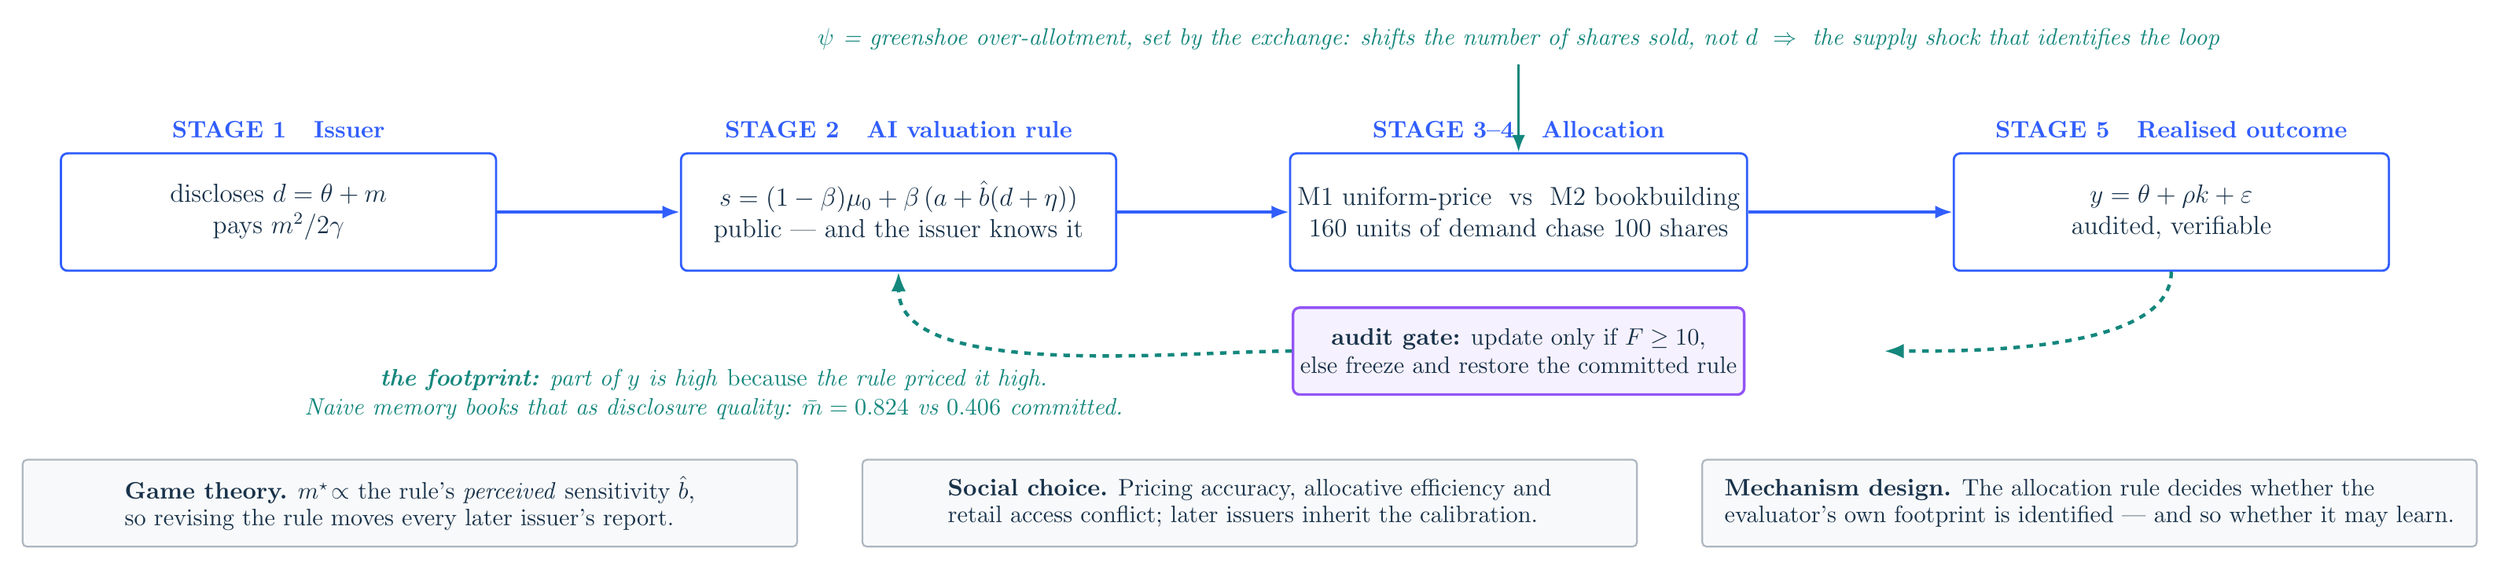
\begin{tikzpicture}[x=1pt,y=1pt,font=\sffamily,>=Latex]
\tikzset{
  stage/.style={draw=CourseBlue,line width=1.0pt,rounded corners=3pt,
                minimum width=200pt,minimum height=54pt,align=center,
                text=CourseInk,fill=white,font=\fontsize{12}{14.5}\selectfont},
  stagelab/.style={font=\bfseries\fontsize{11}{13}\selectfont,text=CourseBlue,align=center},
  flow/.style={CourseBlue,line width=1.3pt,-{Latex[length=8pt]}},
  loop/.style={CourseTeal,line width=1.6pt,-{Latex[length=9pt]},dashed},
  instr/.style={CourseTeal,line width=1.3pt,-{Latex[length=8pt]}},
  gate/.style={draw=CourseViolet,line width=1.2pt,rounded corners=3pt,
               minimum width=186pt,minimum height=40pt,align=center,
               text=CourseInk,fill=CourseViolet!8,font=\fontsize{11}{13}\selectfont},
  note/.style={font=\itshape\fontsize{11}{13.5}\selectfont,text=CourseTeal,align=center},
  lens/.style={draw=CourseInk!35,line width=0.8pt,rounded corners=2pt,
               minimum width=356pt,minimum height=40pt,align=left,
               text=CourseInk,fill=CourseInk!3,font=\fontsize{10.5}{12.5}\selectfont},
  synth/.style={draw=CourseTeal,line width=1.1pt,rounded corners=2pt,
                minimum width=1128pt,minimum height=32pt,align=center,
                text=CourseInk,fill=CourseTeal!4,font=\fontsize{11}{13}\selectfont}
}

% ---------- stage labels -------------------------------------------------
\node[stagelab] at (130,272) {STAGE 1 \ \ Issuer};
\node[stagelab] at (415,272) {STAGE 2 \ \ AI valuation rule};
\node[stagelab] at (700,272) {STAGE 3--4 \ \ Allocation};
\node[stagelab] at (1000,272) {STAGE 5 \ \ Realised outcome};

% ---------- the four stages ---------------------------------------------
\node[stage] (issuer)  at (130,234) {discloses $d=\theta+m$\\pays $m^{2}/2\gamma$};
\node[stage] (rule)    at (415,234) {$s=(1-\beta)\mu_{0}+\beta\,(a+\hat b(d+\eta))$\\public --- and the issuer knows it};
\node[stage] (auction) at (700,234) {M1 uniform-price \ vs \ M2 bookbuilding\\160 units of demand chase 100 shares};
\node[stage] (outcome) at (1000,234) {$y=\theta+\rho k+\varepsilon$\\audited, verifiable};

\draw[flow] (issuer)--(rule);
\draw[flow] (rule)--(auction);
\draw[flow] (auction)--(outcome);

% ---------- the loop, now routed through an audit gate -------------------
\draw[loop] (outcome.south) to[out=-90,in=0,looseness=0.7] (868,170);
\node[gate] (gate) at (700,170) {\textbf{audit gate:} update only if $F\ge10$,\\else freeze and restore the committed rule};
\draw[loop] (gate.west) to[out=180,in=-90,looseness=0.7] (rule.south);
\node[note] at (330,150)
  {\textbf{the footprint:} part of $y$ is high \emph{because} the rule priced it high.\\
   Naive memory books that as disclosure quality: $\bar m=0.824$ vs $0.406$ committed.};

% ---------- the instrument ----------------------------------------------
\draw[instr] (700,302)--(auction.north);
\node[note,anchor=south] at (700,305)
  {$\psi$ = greenshoe over-allotment, set by the exchange: shifts the number of shares sold, not $d$
   $\;\Rightarrow\;$ the supply shock that identifies the loop};

% ---------- three lenses -------------------------------------------------
\node[lens,anchor=west] (l1) at (12,100)
  {\textbf{Game theory.} $m^{\star}\!\propto$ the rule's \emph{perceived} sensitivity $\hat b$,\\
   so revising the rule moves every later issuer's report.};
\node[lens,anchor=west] (l2) at (398,100)
  {\textbf{Social choice.} Pricing accuracy, allocative efficiency and\\
   retail access conflict; later issuers inherit the calibration.};
\node[lens,anchor=west] (l3) at (784,100)
  {\textbf{Mechanism design.} The allocation rule decides whether the\\
   evaluator's own footprint is identified --- and so whether it may learn.};

\end{tikzpicture}}

\caption{The loop we study and the gate we add: disclosure feeds the rule, the rule allocates scarce stock, capital changes outcomes, and outcomes re-enter its history. The gate permits revision only if first-stage $F\ge10$.}
\Description{A five-stage flow across the top: the issuer discloses d equals theta plus m at quadratic cost; the AI valuation rule publishes a public signal s; a uniform-price auction or bookbuilding allocates 100 shares among 160 units of demand and sets the price and proceeds; and the realised outcome y equals theta plus rho times capital plus noise. A dashed arrow runs from the realised outcome back toward the AI rule but passes through an audit gate that only permits the update when the first-stage F statistic is at least ten, otherwise freezing the rule and restoring the last audited parameter. A separate arrow marks the greenshoe shock psi entering the allocation stage as the supply-side instrument. Beneath sit three lens panels for game theory, social choice, and mechanism design.}
\label{fig:teaser}
\end{teaserfigure}
\maketitle\raggedbottom\coursemeta

\begin{figure*}[t]
\centering\scriptsize
\begin{minipage}[t]{0.30\textwidth}\centering
\resizebox{\linewidth}{!}{% Intellectual Merits: annotated research/model diagram.
% Separates INHERITED foundation (grey), our DISTINCT contribution (blue/violet)
% and the SUPPORTING EVIDENCE that backs each contribution claim.
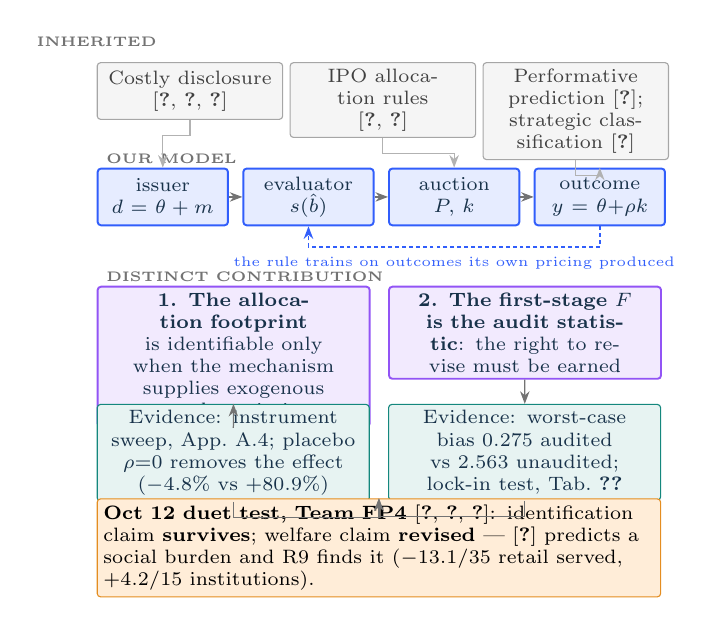
\begin{tikzpicture}[
  font=\scriptsize,
  node distance=0pt,
  box/.style={draw, rounded corners=1.2pt, align=center, inner sep=2.2pt,
              minimum height=7.2mm, line width=0.4pt},
  inherit/.style={box, fill=black!4, draw=black!35, text=black!75},
  ours/.style={box, fill=CourseBlue!12, draw=CourseBlue, text=CourseInk,
               line width=0.7pt},
  evid/.style={box, fill=CourseTeal!10, draw=CourseTeal, text=CourseInk},
  lbl/.style={align=left, font=\tiny\bfseries, text=black!55},
  ar/.style={-{Stealth[length=1.6mm]}, line width=0.45pt, draw=black!55},
  feed/.style={-{Stealth[length=1.6mm]}, line width=0.7pt, draw=CourseBlue,
               dash pattern=on 1.4pt off 1.1pt},
]

% ---- row 1: inherited foundations ---------------------------------------
\node[lbl] (l1) at (0,0) {INHERITED};
\node[inherit, text width=22mm, anchor=north west] (f1) at (0,-2.6mm)
  {Costly disclosure\\\cite{lacker1989,crocker2007,cao2023machine}};
\node[inherit, text width=22mm, anchor=north west] (f2) at (24.5mm,-2.6mm)
  {IPO allocation rules\\\cite{benveniste1989,sherman2005}};
\node[inherit, text width=22mm, anchor=north west] (f3) at (49mm,-2.6mm)
  {Performative prediction \cite{perdomo2020};\\strategic classification \cite{milli2019}};

% ---- row 2: the model chain ---------------------------------------------
\node[lbl, anchor=north west] (l2) at (0,-13mm) {OUR MODEL};
\node[ours, text width=15mm, anchor=north west] (m1) at (0,-16mm)
  {issuer\\$d=\theta+m$};
\node[ours, text width=15mm, anchor=north west] (m2) at (18.5mm,-16mm)
  {evaluator\\$s(\hat b)$};
\node[ours, text width=15mm, anchor=north west] (m3) at (37mm,-16mm)
  {auction\\$P,\,k$};
\node[ours, text width=15mm, anchor=north west] (m4) at (55.5mm,-16mm)
  {outcome\\$y=\theta{+}\rho k$};
\foreach \a/\b in {m1/m2, m2/m3, m3/m4} \draw[ar] (\a) -- (\b);
\draw[feed] (m4.south) -- ++(0,-2.6mm) -| (m2.south)
  node[pos=0.25, below, font=\tiny, text=CourseBlue]
  {the rule trains on outcomes its own pricing produced};

% ---- row 3: distinct contribution + evidence ----------------------------
\node[lbl, anchor=north west] (l3) at (0,-28mm) {DISTINCT CONTRIBUTION};
\node[ours, text width=33mm, anchor=north west, fill=CourseViolet!12,
      draw=CourseViolet] (c1) at (0,-31mm)
  {\textbf{1. The allocation footprint}\\is identifiable only when the
   mechanism supplies exogenous supply variation};
\node[ours, text width=33mm, anchor=north west, fill=CourseViolet!12,
      draw=CourseViolet] (c2) at (37mm,-31mm)
  {\textbf{2. The first-stage $F$ is the audit statistic}: the right to
   revise must be earned};

\node[evid, text width=33mm, anchor=north west] (e1) at (0,-46mm)
  {Evidence: instrument sweep, App.~A.4; placebo $\rho{=}0$ removes the
   effect ($-4.8\%$ vs $+80.9\%$)};
\node[evid, text width=33mm, anchor=north west] (e2) at (37mm,-46mm)
  {Evidence: worst-case bias $0.275$ audited vs $2.563$ unaudited;
   lock-in test, Tab.~\ref{tab:audit}};
\node[box, fill=SdgAmber!18, draw=SdgAmber!90!black, text width=70mm,
      anchor=north west, align=left, font=\scriptsize] (duet) at (0,-58mm)
  {\textbf{Oct 12 duet test, Team FP4} \cite{cao2023machine,perdomo2020,milli2019}:
   identification claim \textbf{survives}; welfare claim \textbf{revised} ---
   \cite{milli2019} predicts a social burden and R9 finds it ($-13.1/35$ retail
   served, $+4.2/15$ institutions).};
\draw[ar] (e1.south) -- ++(0,-2mm) -| (duet.north);
\draw[ar] (e2.south) -- ++(0,-2mm) -| (duet.north);
\draw[ar] (c1) -- (e1);
\draw[ar] (c2) -- (e2);
\draw[ar, draw=black!30] (f1.south) -- ++(0,-2mm) -| (m1.north);
\draw[ar, draw=black!30] (f2.south) -- ++(0,-2mm) -| (m3.north);
\draw[ar, draw=black!30] (f3.south) -- ++(0,-2mm) -| (m4.north);
\end{tikzpicture}
}\\[1pt]
\textbf{(a)} Intellectual Merits: research/model diagram
\end{minipage}\hfill
\begin{minipage}[t]{0.30\textwidth}\centering
\resizebox{\linewidth}{!}{% Practical Impacts: SDG impact diagram.
% Official UN SDG icons are placed ON the diagram. Download the three PNGs from
% https://www.un.org/sustainabledevelopment/news/communications-material/
% into figures/sdg/ as sdg8.png, sdg9.png, sdg16.png. Until they are present
% this file draws a labelled tile in the official goal colour, so the document
% always compiles. Target wording is quoted from https://sdgs.un.org/goals.
\providecommand{\sdgicon}[2]{%
  \IfFileExists{figures/sdg/sdg#1.png}%
    {\includegraphics[width=8.5mm,height=8.5mm]{figures/sdg/sdg#1.png}}%
    {\colorbox{#2}{\parbox[c][7.3mm][c]{7.3mm}{\centering
       \textcolor{white}{\scriptsize\bfseries #1}}}}%
}
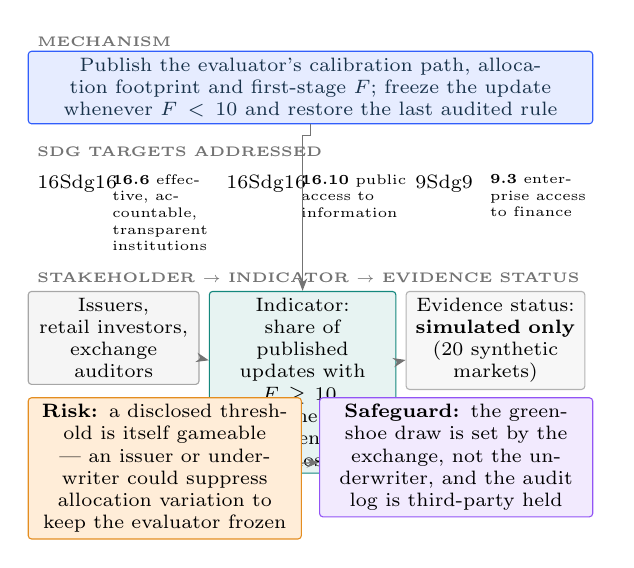
\begin{tikzpicture}[
  font=\scriptsize,
  box/.style={draw, rounded corners=1.2pt, align=center, inner sep=2.4pt,
              minimum height=6.5mm, line width=0.4pt},
  mech/.style={box, fill=CourseBlue!12, draw=CourseBlue, text=CourseInk},
  stake/.style={box, fill=black!4, draw=black!35},
  ind/.style={box, fill=CourseTeal!10, draw=CourseTeal},
  risk/.style={box, fill=SdgAmber!18, draw=SdgAmber!90!black},
  safe/.style={box, fill=CourseViolet!12, draw=CourseViolet},
  lbl/.style={font=\tiny\bfseries, text=black!55, align=left},
  ar/.style={-{Stealth[length=1.6mm]}, line width=0.45pt, draw=black!55},
]

% ---- the mechanism ------------------------------------------------------
\node[lbl, anchor=north west] at (0,0) {MECHANISM};
\node[mech, text width=70mm, anchor=north west] (mech) at (0,-3mm)
  {Publish the evaluator's calibration path, allocation footprint and
   first-stage $F$; freeze the update whenever $F<10$ and restore the last
   audited rule};

% ---- SDG tiles with target codes ---------------------------------------
\node[lbl, anchor=north west] at (0,-14mm) {SDG TARGETS ADDRESSED};
\node[anchor=north west] (i16) at (0,-17.5mm)  {\sdgicon{16}{Sdg16}};
\node[anchor=north west, text width=13.5mm, align=left, font=\tiny]
  at (9.5mm,-17.5mm) {\textbf{16.6} effective, accountable, transparent institutions};
\node[anchor=north west] (i10) at (24mm,-17.5mm) {\sdgicon{16}{Sdg16}};
\node[anchor=north west, text width=13.5mm, align=left, font=\tiny]
  at (33.5mm,-17.5mm) {\textbf{16.10} public access to information};
\node[anchor=north west] (i9) at (48mm,-17.5mm)  {\sdgicon{9}{Sdg9}};
\node[anchor=north west, text width=13.5mm, align=left, font=\tiny]
  at (57.5mm,-17.5mm) {\textbf{9.3} enterprise access to finance};

% ---- the causal chain ---------------------------------------------------
\node[lbl, anchor=north west] at (0,-30mm) {STAKEHOLDER $\rightarrow$ INDICATOR $\rightarrow$ EVIDENCE STATUS};
\node[stake, text width=20mm, anchor=north west] (s1) at (0,-33.5mm)
  {Issuers,\\retail investors,\\exchange auditors};
\node[ind, text width=22mm, anchor=north west] (s2) at (23mm,-33.5mm)
  {Indicator: share of\\published updates with\\$F\!\ge\!10$. Baseline: not\\currently disclosed};
\node[box, text width=21mm, anchor=north west, fill=black!3, draw=black!30]
  (s3) at (48mm,-33.5mm)
  {Evidence status:\\\textbf{simulated only}\\(20 synthetic markets)};
\draw[ar] (s1) -- (s2);
\draw[ar] (s2) -- (s3);

% ---- risk and safeguard -------------------------------------------------
\node[risk, text width=33mm, anchor=north west] (r) at (0,-47mm)
  {\textbf{Risk:} a disclosed threshold is itself gameable --- an issuer or
   underwriter could suppress allocation variation to keep the evaluator frozen};
\node[safe, text width=33mm, anchor=north west] (sf) at (37mm,-47mm)
  {\textbf{Safeguard:} the greenshoe draw is set by the exchange, not the
   underwriter, and the audit log is third-party held};
\draw[ar] (r) -- (sf);
\draw[ar] (mech.south) -- ++(0,-1.4mm) -| (s2.north);
\end{tikzpicture}
}\\[1pt]
\textbf{(b)} Practical Impacts with official SDG icons
\end{minipage}\hfill
\begin{minipage}[t]{0.30\textwidth}\centering
\resizebox{\linewidth}{!}{% NEW for the final project: Future Research Roadmap.
% One unresolved limitation branches into an economics, a computer-science and
% a behavioural-science study. Each carries question / method+data /
% collaborator / progress criterion / milestone.
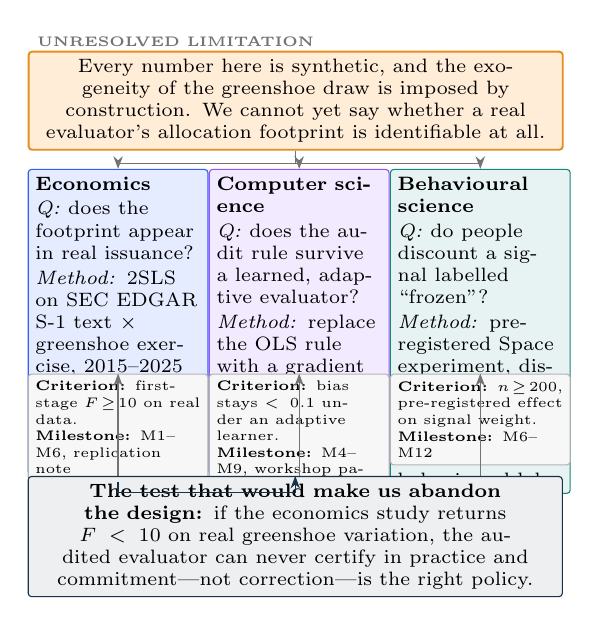
\begin{tikzpicture}[
  font=\scriptsize,
  box/.style={draw, rounded corners=1.2pt, align=left, inner sep=2.6pt,
              line width=0.4pt},
  lim/.style={box, fill=SdgAmber!18, draw=SdgAmber!90!black, align=center,
              text width=66mm, line width=0.7pt},
  econ/.style={box, fill=CourseBlue!12, draw=CourseBlue, text width=21mm},
  cs/.style={box, fill=CourseViolet!12, draw=CourseViolet, text width=21mm},
  beh/.style={box, fill=CourseTeal!10, draw=CourseTeal, text width=21mm},
  mile/.style={box, fill=black!3, draw=black!30, text width=21mm, font=\tiny},
  lbl/.style={font=\tiny\bfseries, text=black!55},
  ar/.style={-{Stealth[length=1.6mm]}, line width=0.45pt, draw=black!55},
]

% ---- the limitation -----------------------------------------------------
\node[lbl, anchor=north west] at (0,0) {UNRESOLVED LIMITATION};
\node[lim, anchor=north west] (lim) at (0,-3mm)
  {Every number here is synthetic, and the exogeneity of the greenshoe draw is
   imposed by construction. We cannot yet say whether a real evaluator's
   allocation footprint is identifiable at all.};

% ---- three studies ------------------------------------------------------
\node[econ, anchor=north west] (e) at (0,-18mm)
  {\textbf{Economics}\\[1pt]
   \textit{Q:} does the footprint appear in real issuance?\\[1pt]
   \textit{Method:} 2SLS on SEC EDGAR S-1 text $\times$ greenshoe exercise,
   2015--2025\\[1pt]
   \textit{Partner:} finance faculty, DKU/Duke Fuqua};
\node[cs, anchor=north west] (c) at (23mm,-18mm)
  {\textbf{Computer science}\\[1pt]
   \textit{Q:} does the audit rule survive a learned, adaptive evaluator?\\[1pt]
   \textit{Method:} replace the OLS rule with a gradient learner; stress-test
   against \cite{perdomo2020}\\[1pt]
   \textit{Partner:} DKU CS; FAccT auditing group \cite{raji2020}};
\node[beh, anchor=north west] (b) at (46mm,-18mm)
  {\textbf{Behavioural science}\\[1pt]
   \textit{Q:} do people discount a signal labelled ``frozen''?\\[1pt]
   \textit{Method:} pre-registered Space experiment, disclosure of audit
   status as treatment\\[1pt]
   \textit{Partner:} DKU behavioural lab};

% ---- criteria and milestones -------------------------------------------
\node[mile, anchor=north west] (me) at (0,-44mm)
  {\textbf{Criterion:} first-stage $F\!\ge\!10$ on real data.\\
   \textbf{Milestone:} M1--M6, replication note};
\node[mile, anchor=north west] (mc) at (23mm,-44mm)
  {\textbf{Criterion:} bias stays $<0.1$ under an adaptive learner.\\
   \textbf{Milestone:} M4--M9, workshop paper};
\node[mile, anchor=north west] (mb) at (46mm,-44mm)
  {\textbf{Criterion:} $n\!\ge\!200$, pre-registered effect on signal weight.\\
   \textbf{Milestone:} M6--M12};

\foreach \a/\b in {e/me, c/mc, b/mb} \draw[ar] (\a) -- (\b);
\draw[ar] (lim.south) -- ++(0,-1.6mm) -| (e.north);
\draw[ar] (lim.south) -- ++(0,-1.6mm) -| (c.north);
\draw[ar] (lim.south) -- ++(0,-1.6mm) -| (b.north);

% ---- the discriminating test -------------------------------------------
\node[box, fill=CourseInk!8, draw=CourseInk, text width=66mm, anchor=north west,
      align=center] (kill) at (0,-57mm)
  {\textbf{The test that would make us abandon the design:} if the economics
   study returns $F<10$ on real greenshoe variation, the audited evaluator can
   never certify in practice and commitment---not correction---is the right
   policy.};
\draw[ar, draw=CourseInk] (me.south) -- ++(0,-1.4mm) -| (kill.north);
\end{tikzpicture}
}\\[1pt]
\textbf{(c)} NEW Future Research Roadmap
\end{minipage}
\caption{Required diagrams; expanded, with full legends, in Appendix~G. SDG icons~\cite{un_sdg,un_sdg_icons}.}
\Description{Three panels side by side. Left: inherited foundations feed a model chain from issuer to evaluator to auction to outcome with a dashed feedback arrow, two violet contribution boxes, two teal evidence boxes and an amber duet-test box. Middle: a mechanism box, three SDG icon tiles for targets 16.6, 16.10 and 9.3, a stakeholder-indicator-evidence chain, and risk and safeguard boxes. Right: an amber limitation box branching into economics, computer-science and behavioural studies with milestones, converging on the abandonment test.}
\label{fig:diagrams}
\end{figure*}

\section{Background}
An AI valuation rule scores an issuer's disclosure, and investors act on the score. Reporters shade against known rules~\cite{lacker1989,crocker2007}, firms write for machine readers~\cite{cao2023machine}, predictors shift what they predict~\cite{perdomo2020}. Unresolved: a rule that \emph{decides a firm's capital}, then retrains on outcomes that capital produced, the Lucas critique~\cite{lucas1976} inside a learning rule.

\section{Motivation}
\textbf{May an exchange let a deployed valuation rule revise itself from outcomes, or must it stay committed?} Backtest accuracy is the statistic a self-influencing rule inflates~\cite{sec2024aiwashing}; our PS2 answer lacked exclusive allocation and sequential rationality (14 October feedback). Missing: a \emph{checkable condition} for safe revision.

\section{Application Scenario}
IPO allocation under real scarcity: 100 shares, 160 units of demand from 15 institutions ($\le6$ each) and 35 retail investors ($\le2$). Stakeholders: issuers, investors, the exchange, later issuers. The exchange-set greenshoe $\psi$ moves shares sold, not disclosure. \textbf{Boundary:} flat demand~\cite{ausubel2014}, no certification effects~\cite{benveniste1989}, synthetic data.

\section{Research Question}
\textbf{Shared question:} \emph{When issuers know the AI evaluator, when may it revise its rule from outcomes it helped cause, and does the allocation mechanism decide?}\\
\textbf{Economics:} how does disclosure respond to the rule's \emph{perceived} sensitivity, and who pays?\\
\textbf{Computation:} can the evaluator separate quality from its own allocation footprint, and when not?\\
\textbf{Behavior:} do investors discount predictable inflation, or over-weight the signal~\cite{logg2019}?

\section{Method}
\textbf{Game.} Issuers $t=1,\dots,N$ arrive in sequence with private $(\theta_t,v_t,\rho_t)$ and disclose $d_t=\theta_t+m_t$ at cost $m_t^2/2\gamma$, earning $v_t\times$proceeds less cost. The evaluator publishes $s_t=(1-\beta)\mu_0+\beta[a+\hat b_t(d_t+\eta_t)]$, $\hat b_t$ public. Investors see $s_t$ and a private $x_{it}=\theta_t+\xi_{it}$ and bid; the mechanism sets price $P_t$ and proceeds $k_t$; $y_t=\theta_t+\rho_tk_t+\varepsilon_t$ enters the history. Incomplete information and sequential moves call for perfect Bayesian equilibrium~\cite{harsanyi1968,fudenberg1991}; beliefs $\mathbb{E}[\theta_t\mid s_t]=\hat d_t-\bar m_t$ are correct on path (sequential rationality: Appendix~A.0), giving
\begin{equation}
m_t^\star=\gamma\,v_t\,n\,\lambda_P\big[\lambda\beta\hat b_t+(1-\lambda)\kappa_0\big].
\label{eq:br}
\end{equation}
\textbf{Lenses} (Fig.~\ref{fig:teaser}). \emph{Game theory:} revising $\hat b$ moves every later report. \emph{Social choice:} accuracy, efficiency and retail access conflict. \emph{Mechanism design}~\cite{myerson1981} decides identification: a naive learner gets
\begin{equation}
\hat b_{\rm naive}=b+\rho\,\operatorname{Cov}(k,d)/\operatorname{Var}(d)+R,
\label{eq:bias}
\end{equation}
whose middle term, the rule's footprint, only a shock to $k$ but not $d$ removes~\cite{pearl1995}. \textbf{Allocation (PS2 comparison retained).} M1 uniform-price: fill from the top, pro-rate the margin, pay the lowest accepted bid~\cite{milgrom1982}; M2 bookbuilding: 85\% to institutions at an 8\% discount; PS2's equal-share rule stays as an arm. \textbf{Memory:} none (committed); naive (OLS); capital-purged (2SLS, $\psi$ instruments $k$); \emph{audited freeze}: purged, revised only if first-stage $F\ge10$~\cite{staiger1997} on $n\ge40$, else the last audited rule returns. \textbf{Design:} 20 seeds $\times$ 4 modes $\times$ 2 mechanisms $\times$ 2 allocation rules; 11 assertions in \texttt{tests/}.

{\footnotesize\smallskip\noindent\textbf{GitHub and tested commit/release:} \GitHubLink\\
\textbf{Runnable notebook:} \NotebookLink\\
\textbf{Hugging Face:} \HuggingFaceLink\\
\textbf{Poster embedded in root README.md:} \PosterLink\par}

\balance
\section{Results}
All results are \textbf{simulated} (20 seeds, $\pm$ 95\% CI); each claim is a test in \texttt{tests/}; frozen run: Appendix~A.

\begin{table}[H]\centering\scriptsize
\caption{Manipulation $\bar m$ and bias $\hat b-b$. RMSE, $F$: Table~\ref{tab:headlinefull}.}
\label{tab:headline}
\setlength{\tabcolsep}{3.5pt}\renewcommand{\arraystretch}{0.95}
\begin{tabular}{@{}lrrrr@{}}\toprule
 & \multicolumn{2}{c}{M1 uniform-price} & \multicolumn{2}{c}{M2 bookbuilding}\\\cmidrule(lr){2-3}\cmidrule(l){4-5}
Memory & $\bar m$ & $\hat b-b$ & $\bar m$ & $\hat b-b$ \\\midrule
No memory      & 0.406\,\tiny$\pm$.00 & 0.000\,\tiny$\pm$.00 & 0.406\,\tiny$\pm$.00 & 0.000\,\tiny$\pm$.00 \\
Naive history  & \textbf{0.824}\,\tiny$\pm$.14 & \textbf{1.030}\,\tiny$\pm$.28 & \textbf{0.717}\,\tiny$\pm$.09 & \textbf{0.768}\,\tiny$\pm$.18 \\
Capital-purged & 0.455\,\tiny$\pm$.09 & 0.090\,\tiny$\pm$.17 & 0.395\,\tiny$\pm$.05 & $-$0.024\,\tiny$\pm$.09 \\
Audited freeze & 0.423\,\tiny$\pm$.06 & \textbf{0.038}\,\tiny$\pm$.14 & 0.416\,\tiny$\pm$.03 & 0.016\,\tiny$\pm$.06 \\\bottomrule
\end{tabular}
\end{table}

\textbf{R1.} Naive history doubles manipulation (M1 $+103\%$, M2 $+77\%$). \textbf{R2.} At $\rho=0$ the lift falls from $+0.328$ to $-0.019$; sign holds in 27/27 settings. \textbf{R3.} Fixing two PS2 defects ($F$ off by $n{-}2$: $0.136$ is $5.47$; a purge reading $b_{\rm true}$), purging works when identified. \textbf{R4.} Below $F=10$ purged bias reaches $-2.563$; the audited worst case is $0.275$, and freezes fall $100\%\!\to\!0\%$ as identification arrives. \textbf{R5.} Without the 40-issuer guard the audit locks in on noise ($-0.362$ vs $0.002$). \textbf{R6.} Inflation compresses bids: M1 excludes 9.5 (naive) vs 17.2 (committed). \textbf{R7--R8.} Negative: $|\mathrm{corr}(k,\rho)|\le0.021$ everywhere; Space data are exploratory. \textbf{R9.} After FP4's challenge via Milli et al.~\cite{milli2019}: versus naive, auditing serves 13.1 fewer of 35 retail investors ($99.9\%\!\to\!62.5\%$), 4.2 more of 15 institutions; not Pareto.

\section{Intellectual Merits}
\emph{(i)} Perdomo et al.~\cite{perdomo2020} ask if retraining under a known shift is \emph{stable}; we ask if the shift is \emph{separable} and show the mechanism decides. \emph{(ii)} Cao et al.~\cite{cao2023machine}: firms adapt to a \emph{fixed} reader; ours retrains on outcomes it caused (Eq.~\eqref{eq:bias}). \emph{(iii)} Milli et al.~\cite{milli2019}: robustness burdens the gamed; it predicted R9. \textbf{Change:} $F$ becomes a governance variable. \textbf{Open:} residual $R$, real greenshoe strength, who bears R9.

\section{Practical Impacts}
\textbf{Mechanism} (Fig.~\ref{fig:diagrams}b): a rule that influences allocation publishes its calibration path, footprint and $F$, and freezes when $F<10$. \textbf{Stakeholders:} issuers, retail investors, auditors. \textbf{Indicator:} share of updates with $F\ge10$ (\textbf{baseline:} none). \textbf{SDG} 16.6 (freeze log), 16.10 (calibration), 9.3 (who is financed). \textbf{Evidence:} intended, simulated. \textbf{Risks/safeguards:} a public threshold is gameable (exchange-set $\psi$, third-party log~\cite{raji2020}); retail pays (publish served share by class). \textbf{Standards:} is $R$ identified, is freezing cheap, who may appeal?

\subsection*{Future Research Roadmap}
Imposed exogeneity drives three studies (Fig.~\ref{fig:diagrams}c). \textbf{Economics:} 2SLS on SEC EDGAR S-1 text $\times$ realised over-allotment, 2015--2025; pass if $F\ge10$. \textbf{CS:} a gradient learner under performative retraining~\cite{perdomo2020}; pass if bias $<0.1$. \textbf{Behavior:} a pre-registered Space study ($n\ge200$) of whether displaced investors find it fair. \textbf{Discriminating test:} a real $F<10$ means we revert to commitment.

\subsection*{Evolving 2056 Contribution Statement}
By 2056, we aspire to advance \emph{identifiability as a licence to learn} for the enduring question of when an institution may trust evidence it helped create. Our current verified contribution is simulated: gating revision on $F\ge10$ cuts worst-case bias from $2.563$ to $0.275$, at a named retail cost. We will test synthetic exogeneity through the EDGAR study, with accountable correction via the freeze log. \textbf{Dated change:} Week~1: can firms fool an AI scorer; PS1: commit or revise; 14 Oct: exclusive allocation; FP4: R9. \textbf{Foundation:} Hall and Woodford's 2026 Prize~\cite{nobel2026} for Lucas-robust microfoundations: our rule is not invariant to its own deployment (2025: App.~G).

\subsection*{Open Science and SDG Statements}
\textbf{Release:} \TestedRelease; MIT licence; synthetic data. \textbf{Shortest run:} \texttt{run\_experiment.py --quick} (40\,s) reproduces Table~\ref{tab:headline}'s signs. \textbf{Limits:} flat demand, exogenous $\rho$, imposed exogeneity. \textbf{SDG evidence needed:} a real $F\ge10$. All artifacts agree.

\subsection*{Final Submission}
\textbf{Wednesday, October 21, 2026, 11:00 p.m. Asia/Shanghai:} paper PDF, Overleaf ZIP, A0 poster PPTX and PDF, plus links and version, once per Canvas group.

\clearpage\balance
\section*{Author Notes}
\subsection*{Full Acknowledgments}
We thank \textbf{Prof. Luyao Zhang} for incubating this project from its strategic-disclosure starting point through PS1 and PS2 to the final submission; for her formal PS1 feedback asking when evaluator memory can substitute for commitment; and in particular for her formal PS2 feedback of 14 October 2026, which identified that our allocation code gave every investor shares and therefore could not exclude anyone, that Section~2 had not supplied the sequential-rationality argument for its equilibrium claim, and that the poster's plotted sensitivities contradicted its headline value. That feedback produced the single largest change in this paper and is the direct cause of result R6. We thank \textbf{Prof. Kenneth S. (Ken) Rogerson}, Program Discussant at the 7 September 2026 \emph{2056 Nobel and Turing Laureate Program Launch Workshop}, for one question: \emph{what makes your AI better than the AI that came before it?} We answered it then in terms of accuracy. The project's central claim is, in effect, a corrected answer --- that the relevant improvement is not predictive but epistemic, a system knowing when it is not entitled to learn --- and the question is the reason we went looking for a criterion rather than a benchmark score. Our contribution-and-question correspondence is recorded in Appendix~G. We thank \textbf{Han Zhang}, Liberata founder and Duke University Ph.D. candidate, for the point that an AI evaluator making consequential errors needs an explicit correction or penalty route rather than being assumed self-correcting --- this became the audited-freeze rule and its restoration criterion. We thank our formal PS2 peer reviewers \textbf{Aaron Wang} (Team FP8) and \textbf{Zhenning Wang}, who independently converged on the same unanswered question --- whether the footprint survives real, possibly endogenous, issuance data --- and on the same remedy, a preregistered replication; that pair of sheets is why the roadmap's first study is an EDGAR replication with a stated abandonment criterion rather than a generic ``future work'' line, and our duet partner \textbf{Team FP4 --- Zhengjun He and Yichen Shen}, who did the project a service twice. Their duet selection of Milli et al.~\cite{milli2019} produced the one external challenge that forced us to \emph{narrow} a claim rather than support it: we had recommended the audited evaluator without measuring who pays for it, and R9 is the result. Their later written points --- clarify how disclosure, allocation and evaluator learning interact; test alternative assumptions and parameter settings; and state how the accountability mechanism would be evaluated in practice --- map directly onto the Method rewrite, Appendix~A's robustness suite, and the Future Research Roadmap. We thank the whole \textbf{COMSCI/ECON 206 classroom community}; every individual who gave us consequential feedback this semester is named above with the specific point they raised, and the standing invitation below covers anyone we have missed. We thank \textbf{Tencent's Shanghai office} and the \textbf{Shanghai Science and Technology Museum} for hosting the field-based learning that framed our public-institution standard~\cite{dku_cscc_2026}.

We build on published work by Lacker and Weinberg~\cite{lacker1989}, Crocker and Slemrod~\cite{crocker2007}, Cao, Jiang, Yang and Zhang~\cite{cao2023machine}, Benveniste and Spindt~\cite{benveniste1989}, Sherman~\cite{sherman2005}, Degeorge, Derrien and Womack~\cite{degeorge2007}, Milgrom and Weber~\cite{milgrom1982}, Ausubel et al.~\cite{ausubel2014}, Perdomo et al.~\cite{perdomo2020}, Staiger and Stock~\cite{staiger1997}, Andrews, Stock and Sun~\cite{andrews2019}, Raji et al.~\cite{raji2020}, Lucas~\cite{lucas1976} and Logg, Minson and Moore~\cite{logg2019}; none of these authors was involved in this work. Software: Python 3.11, NumPy, pandas, Matplotlib, Gradio; the ACM \texttt{acmart} class and the course template as provided. Official SDG icons and target wording are the United Nations'~\cite{un_sdg,un_sdg_icons}; we claim no rights in them. Generative-AI assistance is disclosed in Appendix~A.1. Feedback or a program role does not imply coauthorship. \textbf{Credit check:} we invite any classmate who reviewed this project and is not named above to tell us, and we will correct both the paper and the poster; corrections confirmed to date are recorded in Appendix~D. \emph{This same full list appears on the A0 poster.}

\subsection*{Updated Team and Individual Contributions}
\textbf{Joint contribution.} We produce a checkable condition for when an AI valuation rule may revise itself from outcomes it helped cause: its own capital footprint must be identifiable, measured by the first-stage $F$ of an exchange-set supply shock. The three perspectives change one argument rather than sitting beside it. Economics supplies the objective and the best response that makes rule revision a strategic act; computation turns the condition into a running estimator and a falsifiable test battery; behavioral evidence challenges the rational-investor benchmark the equilibrium rests on. The result neither of us held before this revision is R6: once the offering is genuinely scarce, feedback degrades the auction's capacity to ration, so an accountability failure shows up as an \emph{access} outcome and not only as a pricing error.

\textbf{Feiyu Li.} \emph{Intellectual decision:} to treat the allocation rule as the object that decides whether evaluator learning is admissible at all, rather than as a downstream application --- this reframed Section~4 from a pricing comparison into an identification argument. \emph{Concrete output and location:} the excludable-demand mechanism and the PS2 \texttt{fixed\_rationing} arm (\texttt{src/auction.py}), the issuer and signal primitives (\texttt{src/model.py}), the simulation loop (\texttt{src/simulation.py}), Sections~1--5, the Intellectual Merits and roadmap diagrams. \emph{Verification performed and result:} wrote and ran the four allocation assertions in \texttt{tests/test\_verification.py}; confirmed 16 of 50 investors are excluded at the baseline coverage of 1.6$\times$, that a bid three units below market receives exactly zero, and that the retained PS2 arm still serves all 50 --- establishing that the instructor's criticism is fixed and that the fix is the cause of the change. Feiyu Li also posted the team's first individual self-challenge on 14 October (that the manipulation jump might be an artifact of 200 synthetic issuers) and ran the test that would have confirmed it: the $\rho=0$ placebo, which instead collapsed the lift from $+0.328$ to $-0.019$. \emph{Connection:} the allocation rewrite is what makes R6 and R9 possible and gives the mechanism-design lens something to decide; the placebo is what licenses any causal reading of the feedback effect at all.

\textbf{Xuantong Fu.} \emph{Intellectual decision:} to make the first-stage $F$ the governing statistic of the accountability rule rather than a reported diagnostic --- the evaluator must earn the right to revise. \emph{Concrete output and location:} the 2SLS estimator and the audited-freeze rule with its thick-sample guard (\texttt{src/evaluator.py}), the robustness and falsification suite (\texttt{src/robustness.py}), Appendices~A and~D, Table~\ref{tab:headline}. \emph{Verification performed and result:} re-derived the first-stage statistic and found the PS2 implementation divided by the residual sum of squares rather than the residual variance, understating every reported $F$ by a factor of $n{-}2$ --- recomputing the PS2 artifact gives $5.47$ where the paper reported $0.136$; independently confirmed the estimator no longer reads $b_{\rm true}$ by running it under $b_{\rm true}=1.02$ and $5.00$ and obtaining identical output to nine decimals. Xuantong Fu posted the team's second individual self-challenge on 14 October (that an $F$ of $0.136$ made the correction uninterpretable) and ran the $\sigma_\psi$ sweep it specified, which showed both that the statistic had been mis-normalised and that the underlying worry was right below the threshold. \emph{Connection:} this converted a stated self-challenge into a resolved, conditional finding and supplies the roadmap's abandonment criterion.

\textbf{Documented cross-check.} Each author raised an individual self-challenge and ran the corresponding test, then independently re-ran the other's from a clean checkout. Feiyu re-derived the corrected first-stage statistic and reproduced Xuantong's finding that the legacy formula understates it by a factor of $n-2$, and separately re-ran the audit-lock-in experiment, confirming that removing the 40-issuer guard reproduces a permanent lock-in at a wrong parameter. Xuantong re-ran Feiyu's placebo and confirmed the lift falls from $+0.328$ to $-0.019$ at $\rho=0$, and verified the social-burden decomposition behind R9. Both authors checked that the paper, poster, repository, notebook and Space report the same question, parameters, outputs and evidence labels, and both can explain the complete project.

\bibliographystyle{ACM-Reference-Format}\bibliography{references}
\appendix

\section{Technical Details and Reproducibility}
\textbf{A.0 Sequential rationality and beliefs} (the argument the PS2 draft omitted). The stage game is: nature draws $(\theta_t,v_t,\rho_t)$; the issuer observes them and chooses $m_t$; the evaluator applies its published rule; investors observe $(s_t,x_{it})$ and bid; the mechanism allocates. A PBE is an assessment $(\sigma,\mu)$ such that each player's action is optimal given beliefs at every information set and beliefs follow Bayes' rule on path; we do not impose the full consistency refinement of Kreps and Wilson~\cite{kreps1982}, and say so explicitly.
\emph{(i) Investors.} At their information set an investor knows $s_t$, $x_{it}$, the published $\hat b_t$ and the equilibrium strategy $m^\star(\cdot)$. Inverting the signal gives $\hat d_t$, and subtracting the equilibrium mean inflation $\bar m_t=\mathbb{E}[m^\star(v)]$ gives the belief $\mathbb{E}[\theta_t\mid s_t]=\hat d_t-\bar m_t$, which is Bayes-consistent because $\eta_t$ and $\xi_{it}$ are independent of $v_t$. Precision weighting the public and private components is then sequentially rational for a risk-neutral bidder valuing the asset at $\theta_t$.
\emph{(ii) Issuer.} Taking the investors' linear bidding rule as given, expected proceeds are affine in $d_t$ with slope $n\lambda_P\lambda\beta\hat b_t$, so the issuer solves $\max_m \{n\lambda_P[\lambda\beta\hat b_t+(1-\lambda)\kappa_0]\,m-m^2/2\gamma\}$. The objective is strictly concave, the first-order condition is necessary and sufficient, and it yields Eq.~\eqref{eq:br}. Single crossing holds because the marginal benefit is increasing in $v_t$ while the marginal cost $m/\gamma$ is not, which supports the separating benchmark.
\emph{(iii) Off path.} A disclosure outside the equilibrium range is assigned the belief of the nearest on-path type; because payoffs are continuous and the cost is strictly convex, no type gains from such a deviation, so the assessment survives. \textbf{What this does not claim:} the equilibrium is of the stage game taking $\hat b_t$ as given. We do not claim equilibrium of the full dynamic game in which the evaluator anticipates its own future estimates; that is left open and is the first item a referee should press.

\textbf{A.1 Feedback decomposition.} Substituting $y=\theta+\rho k+\varepsilon$ and $d=\theta+m$ into the naive projection gives Eq.~\eqref{eq:bias}. Verified numerically: on seed~42 the naive slope is $1.847$ against a decomposition prediction of $1.703$ from the measured footprint $\operatorname{Cov}(k,d)/\operatorname{Var}(d)=1.406$, a $7.8\%$ gap attributable to $R$ (\texttt{test\_feedback\_decomposition\_holds}). Note the structural coefficient of $y$ on $d$ holding $k$ fixed is exactly $1.00$, so the stated calibration $b_{\rm true}=1.02$ leaves a perfect estimator with a residual offset near $-0.02$; that offset is a property of the calibration, not of the estimator, and is tested explicitly.

\textbf{A.2 Pseudocode.}
\begin{verbatim}
for seed in 42..61:
 for rule in {excludable, fixed_rationing}:
  for mode in {no_memory, naive, purged, audited}:
   for mech in {uniform_price, bookbuilding}:
    for t in 1..200:
      m   <- best_response(v_t, b_hat)
      d   <- theta_t + m
      s   <- publish(d, b_hat)
      bid <- posterior(s, x_t)         # (price, quantity)
      psi <- greenshoe draw            # exchange-set
      P, alloc, k <- mechanism(bid, psi)   # losers get 0
      y   <- theta_t + rho_t*k + eps
      F   <- first_stage(k ~ 1 + d + psi)
      if mode == audited and (F < 10 or n < 40):
          freeze; b_hat <- last_audited
      else:
          b_hat <- estimate(mode)
\end{verbatim}

\textbf{A.3 Inputs and parameters.} $N=200$ issuers (10 cohorts $\times$ 20), two-cohort burn-in, 100 shares, seeds 42--61. $\sigma_\theta=1.0$, $\gamma=0.006$, $\sigma_\eta=0.5$, $\mu_0=8.5$, $\beta=0.60$, $\lambda=1.0$, $\sigma_\varepsilon=0.8$, $b_{\rm true}=1.02$, $\lambda_P=1.0$, $\kappa_0=0$, $v\sim N(2.2,0.4^2)$, $\rho\sim N(0.50,0.12^2)$ truncated positive. Investors: 15 institutions ($\sigma_\xi=1.0$, max 6 units) and 35 retail ($\sigma_\xi=2.5$, max 2 units), so demand is 160 against a 100-share offering, a coverage ratio of $1.6\times$. Greenshoe s.d. $0.08$ (M1) and $0.20$ (M2); bookbuilding reserves 85\% to institutions at an 8\% discount. Audit threshold $F\ge10$, minimum audit sample 40.

\begin{table}[H]\centering\scriptsize
\caption{Full headline grid behind Table~\ref{tab:headline}, with price RMSE and first-stage $F$ (\texttt{results/headline\_table.csv}).}
\label{tab:headlinefull}
\setlength{\tabcolsep}{3pt}
\begin{tabular}{@{}llrrrr@{}}\toprule
 & Memory & $\bar m$ & RMSE & $\hat b-b$ & $F$ \\\midrule
\multirow{4}{*}{\rotatebox{90}{M1}}
 & No memory      & 0.406\,\tiny$\pm$.00 & 0.45 & 0.000\,\tiny$\pm$.00 & 5939 \\
 & Naive history  & 0.824\,\tiny$\pm$.14 & 8.14 & 1.030\,\tiny$\pm$.28 & 231 \\
 & Capital-purged & 0.455\,\tiny$\pm$.09 & 5.26 & 0.090\,\tiny$\pm$.17 & 36 \\
 & Audited freeze & 0.423\,\tiny$\pm$.06 & 2.57 & 0.038\,\tiny$\pm$.14 & 143 \\\midrule
\multirow{4}{*}{\rotatebox{90}{M2}}
 & No memory      & 0.406\,\tiny$\pm$.00 & 0.78 & 0.000\,\tiny$\pm$.00 & 42537 \\
 & Naive history  & 0.717\,\tiny$\pm$.09 & 4.78 & 0.768\,\tiny$\pm$.18 & 1814 \\
 & Capital-purged & 0.395\,\tiny$\pm$.05 & 1.59 & $-$0.024\,\tiny$\pm$.09 & 2082 \\
 & Audited freeze & 0.416\,\tiny$\pm$.03 & 1.28 & 0.016\,\tiny$\pm$.06 & 5275 \\\bottomrule
\end{tabular}
\end{table}

\textbf{A.4 Robustness and falsification suite} (\texttt{src/robustness.py}). \emph{Placebo:} $\rho=0$ removes the effect ($+0.328\to-0.019$). \emph{Instrument sweep:} $\sigma_\psi\in\{0.01,\dots,0.40\}$; purged bias worst case $-2.563$, audited worst case $0.275$; audited freeze rate falls $99.9\%\to0\%$. \emph{Parameter grid:} $\gamma,\beta,\bar\rho,\sigma_\theta,\sigma_\eta,\sigma_\varepsilon$ one at a time; the manipulation-lift sign holds in 27/27 settings and purging reduces $|{\rm bias}|$ in 27/27. The smallest gain is at $\bar\rho=0.10$ ($0.115\to-0.063$), where the footprint is small enough that correcting it barely matters. \emph{Scarcity sweep:} coverage $1.0\to3.2$. \emph{Audit lock-in:} with and without the thick-sample guard.

\begin{table}[H]\centering\footnotesize
\caption{Audit lock-in. Removing the thick-sample guard lets the rule certify on noise and freeze there permanently.}
\label{tab:audit}
\setlength{\tabcolsep}{4pt}
\begin{tabular}{@{}llrrr@{}}\toprule
Guard & Mech. & $\hat b-b$ & Frozen & RMSE\\\midrule
none ($n_{\min}{=}1$)  & M1 & $-0.362$\,\tiny$\pm$.36 & 58.2\% & 4.73\\
guarded ($n_{\min}{=}40$) & M1 & $\;\;\,0.002$\,\tiny$\pm$.15 & 14.7\% & 2.02\\
none ($n_{\min}{=}1$)  & M2 & $\;\;\,0.004$\,\tiny$\pm$.06 & \;3.9\% & 1.41\\
guarded ($n_{\min}{=}40$) & M2 & $\;\;\,0.021$\,\tiny$\pm$.07 & \;0.0\% & 1.11\\\bottomrule
\end{tabular}
\end{table}

\textbf{A.5 Known limitations.} (1) Flat demand curves: no demand reduction~\cite{ausubel2014}. (2) $\rho$ is exogenous and unobserved by everyone, which is why allocative efficiency on $\rho$ is near zero in every cell (R7; $|r|\le0.021$ across all 16 cells). (3) Memory is cross-firm, an abstraction of repeated calibration. (4) One evaluator, modelled as a rule rather than a strategic vendor. (5) Instrument exogeneity is imposed by construction --- the central unresolved limitation and the roadmap's first target. (6) The residual $R$ in Eq.~\eqref{eq:bias} is unresolved. (7) All data synthetic; no claim about any real issuer. (8) Behavioral evidence is exploratory. (9) The equilibrium is of the stage game, not the full dynamic game (A.0).

\textbf{A.6 Fresh-run record.} \texttt{results/fresh\_run\_record.json} stores the UTC timestamp, seed list, full parameter dump, Python/NumPy/pandas versions, platform string and a SHA-256 prefix for each source file, written by the same command that writes the results. Figures regenerate with \texttt{python src/make\_figures.py}. Tested release: \TestedRelease. \FILL{paste the exact commit SHA, the Space revision hash and the Colab run timestamp here after the final push}.

\subsection{AI Use Disclosure}
AI-Assisted. \textbf{Tools and dates:} OpenAI ChatGPT (GPT-5.6) during September 2026 for LaTeX drafting, Python debugging and interface development, as disclosed in PS2; and Anthropic Claude (Opus 5) on 15 October 2026 for the final revision. \textbf{Bounded purpose of the October session:} re-implementing the allocation mechanism to satisfy the instructor's exclusion criticism, re-deriving the first-stage statistic, building the robustness and falsification suite, generating figures, and drafting LaTeX and poster text. \textbf{Initial independent reasoning:} the authors chose the research question, the strategic environment, the four memory modes, the auction comparison, the social objective and the decision to make identification the governing criterion before any assistance was used; the two self-challenges that drive Appendix~A.4 were written by the authors. \textbf{Material prompts:} the instructor's 14 October feedback, the two author-written self-challenges, and the Zhengjun He / Yichen Shen review, supplied verbatim as the specification to satisfy. \textbf{Accepted:} the excludable-demand implementation, the 2SLS replacement, the thick-sample guard, the placebo and sweep designs, and the figure palette. \textbf{Rejected or revised by the authors:} an initial suggestion to engineer a larger greenshoe variance so the first stage would always pass --- rejected because it would have manufactured the result the test was meant to probe, and replaced by reporting the sweep honestly including the sub-threshold blow-up; and an initial audit rule without a minimum-sample guard, which the authors retained as a \emph{reported failure mode} (Table~\ref{tab:audit}) rather than deleting. \textbf{Human verification:} both authors re-ran the full grid and the 11 assertions from a clean checkout, checked every number quoted in this paper against \texttt{results/headline\_table.csv}, and verified each citation against its DOI. Generative AI was not treated as a source of empirical evidence. The human authors remain responsible for all claims, sources and computation.

\section{Cumulative Intellectual Development}
\textbf{Week 1 --- aspiration.} We asked whether firms could fool an AI scorer. \emph{Consequence:} a question about deception, which the model cannot support, since rational investors de-bias on average.
\textbf{Week 2 --- computational tools and field inquiry.} Field-based learning at Tencent Shanghai and the Shanghai Science and Technology Museum~\cite{dku_cscc_2026} reframed the audience: a claim must be actionable by an institution. \emph{Consequence:} the Practical Impacts standards paragraph distinguishing academic, industry and public criteria.
\textbf{PS1 and instructor feedback.} Prof. Zhang asked when evaluator memory can substitute for commitment. \emph{Consequence:} the fixed-versus-revisable axis that became our four memory modes.
\textbf{ChatGPT Detox workshop; 7 Sept 2026 Launch Workshop.} Prof. Rogerson asked what made our AI better than its predecessors; we answered ``more accurate''. \emph{Consequence:} that answer did not survive contact with the model. Once the evaluator's own allocation enters its training data, accuracy is the statistic it can inflate by itself, so the question pushed us from seeking a better predictor to seeking a condition under which a predictor is \emph{permitted} to update --- which is the paper's thesis and the indicator-and-baseline framing in Practical Impacts.
\textbf{PS2.} We added the allocation mechanism and the learning loop, and reported that purging did not reliably help. \emph{Consequence:} an adverse result we preserved rather than suppressed.
\textbf{Final week --- the consequential change.} The 14 October feedback showed our allocation code could not exclude anyone and that our first-stage statistic was mis-normalised. \emph{Consequence:} the earlier adverse result was a symptom of weak identification, not a property of purging; correcting both produced R3, and the newly scarce offering produced R6, which the PS2 code was structurally incapable of expressing. Our claim moved from ``accountability may not help'' to ``accountability helps exactly when identification holds, and the first stage tells you which regime you are in.''

\section{Open Source and Three Lens Inspiration}
\textbf{Sources and tools.} Python 3.11 (PSF licence), NumPy 1.24 and pandas 2.0 (BSD-3), Matplotlib 3.7 (PSF-based), Gradio (Apache-2.0), ACM \texttt{acmart} (LPPL). \emph{Capability:} exact seeded reproduction of a sequential market. \emph{Limitation:} none provides a weak-instrument-robust estimator, so our inference rests on the first-stage $F$ convention~\cite{staiger1997,andrews2019} and on an exclusion restriction we impose by construction~\cite{pearl1995} rather than on identification-robust confidence sets --- a design consequence we record as a limitation, and the reason the audit rule uses a threshold rather than a continuous penalty. Official SDG icons and target text are UN material~\cite{un_sdg_icons,un_sdg}, used unmodified.
\textbf{Game theory} determines what the issuer does when the rule changes (Eq.~\ref{eq:br}), so it makes rule revision a strategic act rather than a maintenance task. \textbf{Social choice} determines the objective: because later issuers inherit a calibration they never influenced, the welfare criterion is not accuracy, and R6 shows the cost can appear as access rather than price error. \textbf{Mechanism design} determines whether the correction exists at all, since only the allocation rule supplies variation in $k$ orthogonal to $d$. Each lens changes the others: without the mechanism there is no instrument, without the instrument no admissible learning, and without the game-theoretic best response no reason revision would matter.

\section{Feedback Response and Revision Record}
% A description list rather than a tabularx: this record is long and a
% tabularx cannot break across columns or pages.
\begingroup\small
\begin{description}[leftmargin=0pt,labelsep=4pt,style=unboxed,itemsep=4pt]
\item[\textbf{Prof. Luyao Zhang, formal PS2 feedback, 14 Oct 2026}]\ \textbf{Point:} Section~4 and \texttt{src/auction.py} allocate fixed shares, so a bid cannot determine who receives scarce capacity. \textbf{Decision: Revise.} \textbf{Change:} rewrote M1 and M2 with price--quantity bids and 160 units of demand against 100 shares; losers receive zero. PS2 rule retained as the \texttt{fixed\_rationing} arm. \textbf{Location:} \texttt{src/auction.py}; Section~5; Appendix~F. \textbf{Verification:} 4 assertions pass; 16/50 investors excluded at baseline; a bid 3 units below market receives exactly zero; \texttt{results/bid\_trace.json} traces one bid through quantity, price, proceeds and training label as requested. \textbf{Result:} produced R6. \textbf{Author:} Feiyu Li.
\item[\textbf{Prof. Luyao Zhang, 14 Oct 2026}]\ \textbf{Point:} Section~2 does not supply beliefs and a sequential-rationality argument for the equilibrium claim. \textbf{Decision: Revise.} \textbf{Change:} added Appendix~A.0 with investor beliefs, Bayes consistency on path, the issuer's concave problem, single crossing and off-path beliefs; and stated explicitly what is \emph{not} claimed (equilibrium of the full dynamic game). \textbf{Location:} Section~5; Appendix~A.0. \textbf{Author:} Xuantong Fu.
\item[\textbf{Prof. Luyao Zhang, 14 Oct 2026}]\ \textbf{Point:} the poster plots sensitivities near 1.4 while its key message reports about 6.36. \textbf{Decision: Accept.} \textbf{Change:} the two quantities were mean manipulation and a terminal $\hat b$, never labelled as different objects. Every poster and paper number is now regenerated from one frozen 20-seed run into \texttt{results/headline\_table.csv}, and the poster quotes that file only. \textbf{Verification:} paper--poster parity check, Appendix~G. \textbf{Author:} both.
\item[\textbf{Prof. Luyao Zhang, 14 Oct 2026}]\ \textbf{Point:} matching plotted outputs remain unresolved; regenerate from one frozen run. \textbf{Decision: Accept.} \textbf{Change:} single-command pipeline writing a timestamped record with source hashes; figures generated from the same CSVs the paper quotes. \textbf{Location:} \texttt{src/run\_experiment.py}, \texttt{results/fresh\_run\_record.json}.
\item[\textbf{Zhengjun He (Team FP4, with Yichen Shen) --- written challenge in the class thread, 15 October 2026}]\ The three points map onto the three course lenses, and we answer them in that order. \textbf{Point 1:} clarify how strategic disclosure, capital allocation and evaluator learning interact. \textbf{Decision: Revise.} \textbf{Change:} Section~5 now states the interaction as one causal chain and names the exact coupling --- $m^\star$ depends on $\hat b$, $\hat b$ depends on $y$, $y$ depends on $k$, $k$ is set by the mechanism --- and the teaser figure routes the loop through the audit gate. \textbf{Point 2:} test alternative assumptions and parameter settings. \textbf{Decision: Accept.} \textbf{Change:} Appendix~A.4 adds a 27-setting parameter grid, a 7-point instrument sweep, a 7-point scarcity sweep and a placebo, over 20 seeds with CIs. \textbf{Result:} sign robust 27/27. \textbf{Point 3:} clarify how the accountability mechanism would be evaluated in practice and what evidence is needed before policy conclusions. \textbf{Decision: Accept.} \textbf{Change:} Practical Impacts now gives indicator, baseline, evidence status, risk and safeguard, and the roadmap states the EDGAR test and the explicit abandonment criterion. \textbf{Author:} both.
\item[\textbf{Feiyu Li --- individual self-challenge, posted to the class thread 14 October 2026}]\ \textbf{Point, as posted:} ``the $0.408\to1.367$ jump is from 200 fake issuers; if real IPO data does not show it, our story is a model artifact.'' \textbf{Decision: Investigate --- test run.} \textbf{Change:} added the $\rho=0$ placebo, which switches the capital channel off at the source. \textbf{Result:} the lift collapses from $+0.328$ to $-0.019$ ($-4.8\%$), so within the model the effect is the capital channel and not a generic artifact of synthetic data; the sign also holds in 27/27 parameter settings. \textbf{Remaining:} this establishes internal validity only. External validity is the roadmap's economics study, with $F\ge10$ on EDGAR data as the pass criterion. \textbf{Own test, and author:} Feiyu Li --- the author who raised the challenge ran the test.
\item[\textbf{Xuantong Fu --- individual self-challenge, posted to the class thread 14 October 2026}]\ \textbf{Point, as posted:} ``purging reduces bias (4.894 vs 5.344) but the first stage is only 0.136; if a stronger allocation shock still gives a low $F$, the correction does not work and the main claim falls apart.'' \textbf{Decision: Investigate --- test run, claim revised.} \textbf{Change:} ran the instrument sweep the challenge specifies. \textbf{Result:} two findings. First, the $0.136$ was partly a defect --- the statistic divided by the residual sum of squares rather than the residual variance; recomputed on the PS2 artifact it is $5.47$. Second, the substantive worry was still partly right: below $F=10$ the purged estimator is unstable, swinging to $-2.563$. We therefore did not keep the original adverse claim \emph{or} simply reverse it; we replaced it with the conditional claim that purging works when identified and fails unpredictably when not, and made the threshold the rule. \textbf{Own test, and author:} Xuantong Fu --- the author who raised it ran it; independently re-verified by Feiyu Li.
\item[\textbf{Aaron Wang (Team FP8), signed review sheet, 28 September 2026, recommendation Revise}]\ \textbf{Point, verbatim:} ``Behavioral section does not report a completed sample size or actual treatment results''; and the question the evidence could not answer, ``Would the purging method still work if allocation shocks were endogenous in real IPO data?'' The sheet also marked seven checklist items FIX (Appendix~F). \textbf{Decision: Keep the strength, Revise the claim.} \textbf{Change:} behavioral evidence remains labelled exploratory with no population claim (R8); exogeneity is now a stated construction with its own roadmap test rather than an assumption in passing. \textbf{Remaining:} the reviewer's exogeneity question is answered only inside the model --- the greenshoe shock is exogenous by construction. The honest answer is that we cannot settle it here, which is why it is the roadmap's first study with a stated abandonment criterion. \textbf{Strength preserved:} the cited strength (Fig.~2's memory-versus-manipulation contrast) survived every robustness check and is retained as R1.
\item[\textbf{Zhenning Wang, signed review sheet, 28 September 2026, recommendation Investigate}]\ \textbf{Point, verbatim:} ``All data are synthetic, so the 73\% increase may not generalise to real IPO markets''; and ``Does the same footprint bias persist when tested on real issuance data with heterogeneous issuers?'' The sheet marked three checklist items FIX, including players/actions/payoffs/timing/information with a justified solution concept --- the same gap the instructor identified six weeks later, which we had not closed in between. \textbf{Decision: Investigate.} \textbf{Change:} the parameter grid varies issuer-side heterogeneity ($\sigma_\theta$, $\bar\rho$, $\gamma$) over 27 settings and 10 seeds. \textbf{Result:} the effect's sign and the correction's usefulness both survive everywhere, but the \emph{magnitude} does not --- the naive bias ranges from $0.095$ at $\bar\rho=0.10$ to $23.98$ at $\bar\rho=1.00$, a 250-fold spread. That supports the reviewer's point about magnitude while not supporting a claim that the mechanism is an artifact. \textbf{Reasoned disagreement, preserved:} we do not accept that synthetic evidence is uninformative here, because the placebo isolates the mechanism; we do accept it cannot establish magnitude, and we claim none.
\item[\textbf{Han Zhang, Liberata}]\ \textbf{Point:} a failing AI evaluator needs an explicit correction or penalty route. \textbf{Decision: Adapt --- now implemented and tested, not proposed.} \textbf{Change:} the audited-freeze mode with an explicit freeze criterion ($F<10$ or $n<40$) and restoration criterion (restore the last audited parameter; resume automatically once identified). \textbf{Result:} worst-case bias $0.275$ vs $2.563$; and we report its failure mode (Table~\ref{tab:audit}). \textbf{Remaining:} who may appeal a frozen rule is a governance question we raise but do not answer.
\item[\textbf{Team FP4 --- Zhengjun He and Yichen Shen, Oct 12 duet}]\ \textbf{Point:} selected Cao et al.~\cite{cao2023machine}, Perdomo et al.~\cite{perdomo2020} and Milli et al.~\cite{milli2019} as the three closest works, the third on the ground that it covers ``the welfare and fairness costs of strategic adaptation'' against our ``issuer manipulation, allocation efficiency, and the different effects on issuers and investors''. \textbf{Decision: Revise --- claim narrowed.} \textbf{Why:} Milli et al.\ prove that a gain in institutional utility from strategy-robustness is matched by a social burden on those classified. Our audited-freeze rule is exactly such a device, and we had asserted its benefit without measuring who paid for it. \textbf{Change:} added the served-share-by-class decomposition (\texttt{social\_burden} in \texttt{src/run\_experiment.py}), reported as R9; added a second risk and safeguard to Practical Impacts; extended the roadmap's behavioural study to ask whether displaced participants judge the rule fair; and qualified the 2056 statement. \textbf{Verification:} on the frozen 20-seed grid the audited rule serves $13.1$ fewer of 35 retail investors ($99.9\%\to62.5\%$) and $4.2$ more of 15 institutions ($36.7\%\to64.8\%$) than the unsafeguarded rule; \texttt{results/social\_burden.csv}, checked by \texttt{tools/check\_numbers.py}. \textbf{Result:} we no longer claim the audited rule is an improvement full stop; we claim it is an integrity gain with a named distributional price. \textbf{Author:} Feiyu Li ran the decomposition; Xuantong Fu verified it.
\item[\textbf{Oct 14--15 roundtable and class thread --- Zhengjun He and Yichen Shen (Team FP4)}]\ \textbf{Points, one per lens.} \emph{Strategic thinking:} explain more clearly how strategic disclosure, capital allocation and evaluator learning interact. \emph{Mechanism design and computation:} test alternative assumptions and parameter settings to establish robustness beyond the current simulation. \emph{Social choice and welfare:} clarify how the accountability mechanism would be evaluated in practice and what evidence is needed before drawing policy conclusions. \textbf{Decision: Accept all three.} \textbf{Changes:} Section~5 states the coupling as one chain with each dependency named; Appendix~A.4 adds the placebo, a 27-setting parameter grid and two sweeps over 10--20 seeds with CIs; Practical Impacts now carries indicator, baseline, evidence status and two risk/safeguard pairs, and the roadmap states the discriminating test and the abandonment criterion. \textbf{Verification:} sign robust 27/27; purge helps 27/27; \texttt{tools/check\_numbers.py} ties every quoted figure to the frozen run. \textbf{Result:} the third point, taken together with FP4's duet selection of Milli et al.~\cite{milli2019}, is what produced R9. \textbf{Authors:} Xuantong Fu (robustness suite), Feiyu Li (burden decomposition). No further roundtable challenges were raised by classmates outside Team FP4.
\end{description}\endgroup

\smallskip\noindent\textbf{Response status.} Every consequential comment above is answered with a code change, a run, or an explicitly bounded next test. Two prior claims were revised rather than defended: the PS2 adverse purging result (now conditional on identification) and the PS2 first-stage figure (a defect, corrected and documented). One prior strength survived challenge and is preserved: the core feedback effect, which the placebo confirms.

\clearpage\nobalance\onecolumn
\section{Structured Abstract and Cumulative Proposal Map}
\begin{table}[H]\caption{The eight required parts and the consequential final revision.}
\renewcommand{\arraystretch}{1.10}
\begin{tabularx}{\textwidth}{@{}p{0.20\textwidth}Y@{}}\toprule
\textbf{Part}&\textbf{Current statement and revision evidence}\\\midrule
Background & An AI rule that both scores a firm and influences its capital later retrains on outcomes that capital produced. Foundations: costly disclosure~\cite{lacker1989,crocker2007,cao2023machine}, performative prediction~\cite{perdomo2020}, IPO allocation~\cite{benveniste1989,sherman2005}. Unresolved: no checkable condition for when such revision is safe.\\
Motivation & An exchange must decide whether a deployed rule may revise itself. Backtest accuracy is the wrong criterion because a self-influencing rule inflates it.\\
Application Scenario & Sequential IPO allocation: 100 shares, 160 units of demand, 15 institutions and 35 retail, exchange-set greenshoe. Boundary: flat demand curves, no certification effects, synthetic data.\\
Research Question & Under what condition may an AI evaluator revise itself from outcomes it caused, and does the allocation mechanism decide whether that condition can hold?\\
Method & PBE~\cite{harsanyi1968,fudenberg1991} with beliefs and sequential rationality in Appendix~A.0; four memory modes; M1 uniform-price with exclusion vs M2 bookbuilding, plus the retained PS2 fixed-rationing arm; 20 seeds $\times$ 4 modes $\times$ 2 mechanisms $\times$ 2 rules.\\
Results & \textbf{Simulated.} Naive history doubles manipulation ($0.406\to0.824$, M1); placebo $\rho=0$ removes it ($-4.8\%$); purging works when identified (bias $1.030\to0.090$); below $F=10$ it is unstable ($-2.563$) while the audited rule's worst case is $0.275$; without a thick-sample guard the audit locks in; feedback degrades rationing (R6); allocative efficiency on $\rho$ is near zero everywhere (R7, negative). Verified by 11 assertions.\\
Intellectual Merits & Against Perdomo et al.~\cite{perdomo2020}, Benveniste--Spindt~\cite{benveniste1989} and Cao et al.~\cite{cao2023machine}: the first-stage $F$ becomes a governance variable, not a diagnostic. Unresolved: residual $R$; real-data identifiability.\\
Practical Impacts & Publish the calibration path, footprint and $F$; freeze when $F<10$. Targets 16.6, 16.10, 9.3. Indicator: share of updates with $F\ge10$; baseline: not currently disclosed. Evidence status: intended benefit, simulated only. Risk: a disclosed threshold is gameable. Safeguard: exchange-set shock, third-party audit log.\\
Future Research Roadmap & Economics (EDGAR 2SLS), computer science (adaptive learner), behavioural (pre-registered Space study), each with criterion and milestone; abandonment criterion stated in advance.\\
\bottomrule
\end{tabularx}\end{table}

\section{Retained PS2 Auction Artifact and Symposium Record}
\textbf{Rules, stated explicitly.} \emph{M1 uniform-price.} Scarce resource: 100 shares plus an exchange-set over-allotment $\psi$. Participants: 15 institutions ($\sigma_\xi=1.0$, up to 6 units) and 35 retail ($\sigma_\xi=2.5$, up to 2 units). Values/signals: common value $\theta$, private signal $x_i$, public signal $s$. Bids: price--quantity pairs from the posterior mean. Allocation: rank by price, fill until the offering is exhausted, pro-rate the marginal bidder, \emph{exclude everyone below the clearing bid}. Payment: lowest accepted bid. Stopping: cumulative demand reaches the offering. \emph{M2 bookbuilding.} Allocation: 85\% reserved to institutions, scarce within each tranche. Payment: 8\% discount to the precision-weighted institutional estimate. Stopping: close of the book. \emph{Retained PS2 arm.} Equal shares to all 50 investors, nobody excluded, clearing at the lowest bid --- preserved so the September evidence stays inspectable.

\textbf{Predicted vs actual.} Predicted: making the offering excludable would change \emph{who} is financed without changing the sign of the feedback effect. Actual: confirmed on both counts. The headline sign is unchanged against the retained arm (naive-history $\bar m$ $0.824$ excludable vs $0.817$ fixed-rationing), while exclusion and retail share --- constant by construction in PS2 at 0 and 70.0\% --- now move with the memory mode (R6). \textbf{One bid traced} (\texttt{results/bid\_trace.json}), as requested: raising the marginal investor's bid by one unit takes their quantity from 0 to 2 units, moves the clearing price and proceeds, and therefore changes the training label $y=\theta+\rho k$ the evaluator later learns from. That chain is the point of the mechanism in this paper.

\textbf{Analogy boundary.} Real bookbuilding involves certification, relationship allocation and laddering~\cite{degeorge2007}; real multi-unit bidders shade demand~\cite{ausubel2014}; real greenshoe exercise is an underwriter decision, which is precisely why we assign it to the exchange and flag the assumption as the roadmap's first test.

\textbf{September 28 presentation and formal peer review.} Two signed review sheets were received at the 28 September symposium (Session~C) and are retained with the submission.

\emph{Sheet 1 --- Aaron Wang (Team FP8, member 1), dated 28 September, recommendation \textbf{Revise}.} \emph{Strength to retain:} ``Fig.~2 clearly shows how naive memory increases manipulation and how purging reduces bias.'' \emph{Priority concern:} ``Behavioral section does not report a completed sample size or actual treatment results.'' \emph{Genuine question the evidence cannot answer:} ``Would the purging method still work if allocation shocks were endogenous in real IPO data?'' \emph{Feasible verification step:} ``Run with a preregistered sample.'' \emph{Checklist items marked FIX:} member forks and merged pull requests; README identifying a tested commit, run steps and reproduced outputs; Space and GitHub using matching rules and parameters; paper/poster/repository/Space agreeing on authors, claim and evidence status; poster academic block; prediction-versus-observed with a valid completed $n$; and the concrete real-world case with stakeholders, risks, access/correction and an SDG target.

\emph{Sheet 2 --- Zhenning Wang, recommendation \textbf{Investigate}.} \emph{Strength to retain:} ``Game rules, payoff matrix, equilibrium analysis. Figures 1--2 clearly show self-calibration overestimates disclosure quality and increases manipulation under different mechanisms.'' \emph{Priority concern:} ``Not yet LLM-advice / classroom-play data, behavioral claim remains theoretical. All data are synthetic, so the 73\% increase may not generalise to real IPO markets.'' \emph{Genuine question:} ``Does the same footprint bias persist when tested on real issuance data with heterogeneous issuers?'' \emph{Feasible verification step:} ``Run preregistered replication on real IPO data, update Figure~2.'' \emph{Checklist items marked FIX:} README tested commit; players, actions, payoffs, timing and information with a justified solution concept; and matched benchmark with computed result, metric, uncertainty and limitation matching the tested code.

\emph{Disposition of every FIX item.} Tested commit and reproduced outputs: \texttt{results/fresh\_run\_record.json} now records seeds, parameters, library versions and a per-file hash, written by the same command that writes the results. Space/GitHub parameter parity and artifact agreement: enforced mechanically by \texttt{tools/check\_numbers.py}, which fails if any figure quoted in the paper, poster or README drifts from the frozen run. Poster academic block: title, both authors, affiliation, course and instructor, team ID, version, full acknowledgments, named contributions and references are all present on the A0 sheet. Players, actions, payoffs, timing, information and justified solution concept: Appendix~A.0, which is also what the instructor's 14 October feedback required. Benchmark with uncertainty and limitation: 20 seeds with confidence intervals computed across seeds, plus nine stated limitations. Completed $n$ for the behavioural claim: \emph{not supplied}; the claim is withdrawn to exploratory status (R8) rather than asserted. Real-world case with SDG target and metric: the Practical Impacts section now carries mechanism, stakeholders, indicator, baseline, evidence status and two risk/safeguard pairs. Member forks and merged pull requests: \FILL{confirm both personal forks and merged PRs are visible in the org repository before the final push}.

\emph{Both reviewers converged on the same unanswered question} --- whether the footprint survives real, possibly endogenous, issuance data --- and both proposed the same verification, a preregistered replication. That is now the first study in the Future Research Roadmap, with $F\ge10$ on EDGAR data as its pass criterion and an explicit abandonment rule. The full author response to each reviewer is in Appendix~D.

\textbf{Parity check.} Paper, GitHub, Colab, Space and poster share one question, one parameter set, one results file (\texttt{results/headline\_table.csv}) and one set of evidence labels. The Space exposes the same decision --- disclosure, AI valuation, investor action, allocation --- and states on its landing page that its evidence is exploratory.

\section{Final Week Evidence and Final Release Audit}
\textbf{Oct 12 (Theory and Practice). Duet partner: Team FP4 --- Zhengjun He and Yichen Shen.}

\emph{The three closest papers FP4 selected to challenge us, with their stated reasons.} \textbf{(1)} Cao, Jiang, Yang and Zhang~\cite{cao2023machine}, \emph{Review of Financial Studies} 36(9), 3603--3642, \texttt{10.1093/rfs/hhad021} --- ``both examine how firms strategically adjust disclosures in response to AI-based evaluation''; theirs empirical, ours a model linking manipulation to IPO capital allocation. \textbf{(2)} Perdomo, Zrnic, Mendler-D\"unner and Hardt~\cite{perdomo2020}, ICML, PMLR 119, 7599--7609 --- ``both study prediction systems that change the outcomes they later use as training data''; performative stability matches our concern that the rule learns from outcomes its own allocation produced. \textbf{(3)} Milli, Miller, Dragan and Hardt~\cite{milli2019}, FAT*~'19, 230--239, \texttt{10.1145/3287560.3287576} --- ``both examine how firms strategically respond to algorithmic decision rules'', with Milli et al.\ focused on the welfare and fairness cost of strategic adaptation.

\emph{Claims we put up for challenge.} (C1) the allocation claim: a change in a bid changes who is served, which the PS2 code could not support; (C2) the equilibrium claim: the PBE is supported by stated beliefs and sequential rationality (Appendix~A.0); (C3) the welfare claim: gating revision on identification improves the outcome.

\emph{Outcome, and the evidence each challenge required.} C1 and C2 survive: FP4's (1) and (2) establish that firms adapt and that predictors are performative, but neither supplies an \emph{admissibility condition} for outcome-based revision, which is our contribution; the evidence we supplied is \texttt{results/bid\_trace.json} and Appendix~A.0. \textbf{C3 did not survive and we revised it.} FP4's (3) is a theorem about us: Milli et al.\ prove that any institutional gain from strategy-robustness is matched by a social burden on the classified, concentrated on the disadvantaged. Our audited-freeze rule is such a device and we had not measured its burden. The evidence needed was a served-share decomposition by investor class, which we then ran on the frozen 20-seed grid: relative to the unsafeguarded rule the audited evaluator serves $13.1$ fewer of 35 retail investors and $4.2$ more of 15 institutions (R9; \texttt{results/social\_burden.csv}). The Practical Impacts risk register, the roadmap's behavioural study and the 2056 statement were all changed as a result. This is the single most consequential external challenge the project received.

Course Ed thread: \url{https://edstem.org/us/courses/102917/discussion/8381683?comment=19460396}. \FILL{the Category~I / II / III synthesis posts (ours: 1 Intellectual Merits, 2 Practical Impacts, 3 Future Research Roadmap; partner sections 4 Literature and Defense, 5 Potential SDGs, 6 Award and Our Support; unnumbered Acknowledgments); the confirmed author responses added live during the defence; takeaway sheet and handwritten exit}.

\textbf{Oct 14 (Research and Innovation).} Revised poster confirmed embedded in the root \texttt{README.md} with a working PDF link. \emph{Individual self-challenge questions, posted to the class thread on 14 October 2026.} \textbf{Feiyu Li} posted: ``We claim that a history-aware AI causes way more manipulation (0.408 to 1.367 in Fig 2), but this is just from 200 fake issuers with no real data. If real IPO data doesn't show the same jump, our whole story is just a model artifact.'' \emph{Test run:} the $\rho=0$ placebo, which switches the capital channel off at its source and would have confirmed the artifact reading had the effect survived. \emph{Result:} the manipulation lift collapses from $+0.328$ to $-0.019$, so within the model the effect is the capital channel; external validity is deferred to the roadmap's EDGAR study with $F\ge10$ as the pass criterion. \textbf{Xuantong Fu} posted: ``We say the purged-memory rule reduces bias under uniform-price (4.894 vs 5.344 in the M1 table), but the first-stage F is only 0.136, which is really weak. If a stronger allocation shock still gives a low F, then our correction doesn't actually work and the main claim falls apart.'' \emph{Test run:} the $\sigma_\psi$ sweep the challenge specifies. \emph{Result:} two findings --- the $0.136$ was partly a normalisation defect (correctly computed, $5.47$), and the substantive worry was partly right, since below $F=10$ the purged estimator is unstable ($-2.563$). The claim was replaced rather than defended. Each author independently re-ran the other's test from a clean checkout. \emph{Assigned responses to classmates.} Both authors replied to Zhengjun He's review in the course Ed thread (\url{https://edstem.org/us/courses/102917/discussion/8381683?comment=19460396}), deliberately splitting the three points so the two responses are not interchangeable. \textbf{Feiyu Li} answered the interaction point and the distributional half of the practice point, reporting the rewritten allocation chain with the traced bid, and the R9 burden decomposition, and asking FP4 in return whether a retail allocation obtained at a distorted price should count as access at all. \textbf{Xuantong Fu} answered the robustness point and the evidence point, reporting the 27-setting grid, the seed-level confidence intervals, the mis-normalised first-stage statistic flagged in the self-challenge, and the EDGAR abandonment criterion, and conceding that the exchange-set shock does not fully close the gaming risk a published threshold creates. Posted on Ed by Feiyu Li on 15 October 2026 and by Xuantong Fu on 16 October 2026; the texts as posted are in \texttt{docs/ED\_REPLIES.md}. \emph{Challenges received, and what each produced.} Team FP4 --- \textbf{Zhengjun He} and \textbf{Yichen Shen} --- raised three, one per lens. \textbf{Strategic thinking:} ``the theoretical framework would benefit from a clearer explanation of how strategic disclosure, capital allocation, and evaluator learning interact.'' \emph{Revision:} Section~5 now states the coupling as one chain with the dependency named at each link ($m^\star$ on $\hat b$, $\hat b$ on $y$, $y$ on $k$, $k$ on the mechanism), and the teaser routes the loop through the audit gate. \textbf{Mechanism design and computation:} ``consider testing alternative model assumptions and parameter settings to establish how robust the results are beyond the current simulation setup.'' \emph{Revision:} Appendix~A.4 adds a 27-setting parameter grid, a 7-point instrument sweep, a 7-point scarcity sweep and the $\rho=0$ placebo, over 10--20 seeds with confidence intervals; the sign survives 27/27. \textbf{Social choice and welfare:} ``clarify how the proposed accountability mechanism could be evaluated in practice and what additional evidence is needed before drawing policy conclusions.'' \emph{Revision --- the consequential one:} this forced us to ask who pays for the safeguard, which together with FP4's duet selection of Milli et al.~\cite{milli2019} produced R9 and the second risk/safeguard pair in Practical Impacts. The indicator (share of published updates with $F\ge10$), its baseline (not currently disclosed anywhere), and the evidence still missing (real greenshoe variation clearing $F\ge10$) are now stated rather than implied. No further challenges were raised verbally at the roundtable by classmates outside Team FP4. \textbf{The adverse safeguard result, explained as asked:} our PS2 finding that purging could worsen the comparison was not a property of purging but of identification --- under the PS2 mechanism the first stage was weak, so the correction was estimated on variation that barely existed. The test that would make us abandon our preferred design is stated in advance in the roadmap: $F<10$ on real greenshoe variation. The freeze criterion is $F<10$ or $n<40$; the restoration criterion is to reinstate the last audited parameter and resume automatically once the first stage recovers.

\textbf{Contribution/question email to Prof. Ken Rogerson.} Each author sent a separate message to \texttt{rogerson@duke.edu} from their own DKU account, with a distinct contribution and a distinct question: Feiyu Li asked whether a publicly declared freeze is survivable for a real institution, and Xuantong Fu asked what keeps a published self-assessment threshold from becoming a target to be managed rather than met. Both emails were sent on 16 October 2026; copies of the sent messages are retained, and the texts are in \texttt{docs/ROGERSON\_EMAIL.md}; it introduces the authors and team, names COMSCI/ECON 206 and Prof. Luyao Zhang, cites his role as Program Discussant at the 7 September 2026 2056 Nobel and Turing Laureate Program Launch Workshop, thanks him for the specific question he put to us there (what makes your AI better than the AI that came before it), gives the corrected answer the project produced, describes each author's own verified contribution, and asks one question connected to the roadmap --- whether a publicly declared freeze is survivable for a real institution.

\textbf{2026 Nobel verification and comparison with 2025.} Verified from the official announcement: the 2026 Prize in Economic Sciences was awarded on 12 October 2026 to Robert E. Hall and Michael Woodford ``for microeconomic foundations of macroeconomic stabilisation''~\cite{nobel2026}; the 2025 Prize went to Joel Mokyr, Philippe Aghion and Peter Howitt ``for having explained innovation-driven economic growth''~\cite{nobel2025}. \textbf{Resulting change to our 2056 statement:} the 2026 citation gave us a sharper name for our own failure mode. A reduced-form evaluator estimated on past outcomes is exactly the kind of non-invariant relationship the Lucas critique~\cite{lucas1976} warns against and that microfounded modelling was built to repair; our rule fails because it is not invariant to its own deployment. We therefore narrowed the 2056 statement from the vaguer ``auditable AI valuation'' to ``identifiability as a licence to learn''. The 2025 Prize supplies the contrast that makes the point precise: creative destruction~\cite{aghion1992} is a case where changing the world is the goal, whereas our evaluator's problem is that it changes the world and then reads the change as neutral evidence about itself. Our research question and results are unchanged by this comparison; only the 2056 framing moved. Official sources are cited above.

\textbf{Three diagrams, expanded.} The three panels of Figure~\ref{fig:diagrams} appear compactly in the main text and full-width below, each with its explanation, legend and full references. SDG targets and icons match the proposed mechanism and the declared evidence status (intended benefit, simulated only).

\begin{figure}[H]\centering
\resizebox{0.86\textwidth}{!}{% Intellectual Merits: annotated research/model diagram.
% Separates INHERITED foundation (grey), our DISTINCT contribution (blue/violet)
% and the SUPPORTING EVIDENCE that backs each contribution claim.
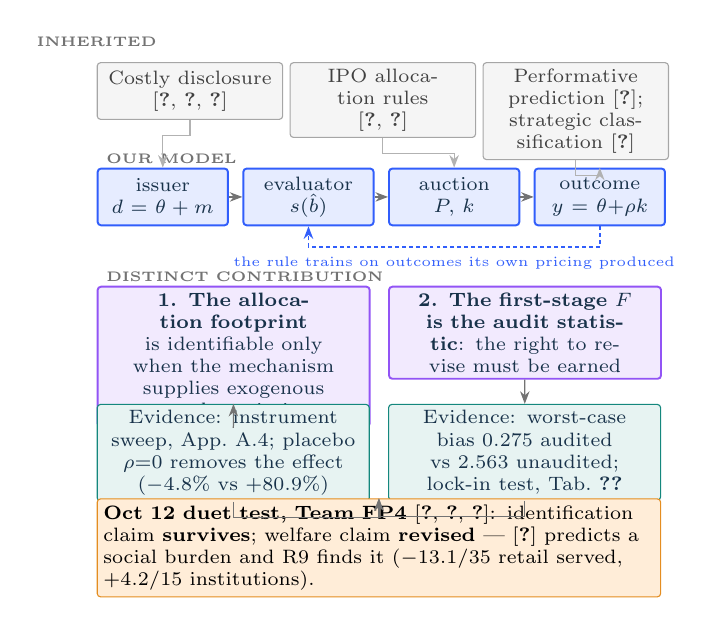
\begin{tikzpicture}[
  font=\scriptsize,
  node distance=0pt,
  box/.style={draw, rounded corners=1.2pt, align=center, inner sep=2.2pt,
              minimum height=7.2mm, line width=0.4pt},
  inherit/.style={box, fill=black!4, draw=black!35, text=black!75},
  ours/.style={box, fill=CourseBlue!12, draw=CourseBlue, text=CourseInk,
               line width=0.7pt},
  evid/.style={box, fill=CourseTeal!10, draw=CourseTeal, text=CourseInk},
  lbl/.style={align=left, font=\tiny\bfseries, text=black!55},
  ar/.style={-{Stealth[length=1.6mm]}, line width=0.45pt, draw=black!55},
  feed/.style={-{Stealth[length=1.6mm]}, line width=0.7pt, draw=CourseBlue,
               dash pattern=on 1.4pt off 1.1pt},
]

% ---- row 1: inherited foundations ---------------------------------------
\node[lbl] (l1) at (0,0) {INHERITED};
\node[inherit, text width=22mm, anchor=north west] (f1) at (0,-2.6mm)
  {Costly disclosure\\\cite{lacker1989,crocker2007,cao2023machine}};
\node[inherit, text width=22mm, anchor=north west] (f2) at (24.5mm,-2.6mm)
  {IPO allocation rules\\\cite{benveniste1989,sherman2005}};
\node[inherit, text width=22mm, anchor=north west] (f3) at (49mm,-2.6mm)
  {Performative prediction \cite{perdomo2020};\\strategic classification \cite{milli2019}};

% ---- row 2: the model chain ---------------------------------------------
\node[lbl, anchor=north west] (l2) at (0,-13mm) {OUR MODEL};
\node[ours, text width=15mm, anchor=north west] (m1) at (0,-16mm)
  {issuer\\$d=\theta+m$};
\node[ours, text width=15mm, anchor=north west] (m2) at (18.5mm,-16mm)
  {evaluator\\$s(\hat b)$};
\node[ours, text width=15mm, anchor=north west] (m3) at (37mm,-16mm)
  {auction\\$P,\,k$};
\node[ours, text width=15mm, anchor=north west] (m4) at (55.5mm,-16mm)
  {outcome\\$y=\theta{+}\rho k$};
\foreach \a/\b in {m1/m2, m2/m3, m3/m4} \draw[ar] (\a) -- (\b);
\draw[feed] (m4.south) -- ++(0,-2.6mm) -| (m2.south)
  node[pos=0.25, below, font=\tiny, text=CourseBlue]
  {the rule trains on outcomes its own pricing produced};

% ---- row 3: distinct contribution + evidence ----------------------------
\node[lbl, anchor=north west] (l3) at (0,-28mm) {DISTINCT CONTRIBUTION};
\node[ours, text width=33mm, anchor=north west, fill=CourseViolet!12,
      draw=CourseViolet] (c1) at (0,-31mm)
  {\textbf{1. The allocation footprint}\\is identifiable only when the
   mechanism supplies exogenous supply variation};
\node[ours, text width=33mm, anchor=north west, fill=CourseViolet!12,
      draw=CourseViolet] (c2) at (37mm,-31mm)
  {\textbf{2. The first-stage $F$ is the audit statistic}: the right to
   revise must be earned};

\node[evid, text width=33mm, anchor=north west] (e1) at (0,-46mm)
  {Evidence: instrument sweep, App.~A.4; placebo $\rho{=}0$ removes the
   effect ($-4.8\%$ vs $+80.9\%$)};
\node[evid, text width=33mm, anchor=north west] (e2) at (37mm,-46mm)
  {Evidence: worst-case bias $0.275$ audited vs $2.563$ unaudited;
   lock-in test, Tab.~\ref{tab:audit}};
\node[box, fill=SdgAmber!18, draw=SdgAmber!90!black, text width=70mm,
      anchor=north west, align=left, font=\scriptsize] (duet) at (0,-58mm)
  {\textbf{Oct 12 duet test, Team FP4} \cite{cao2023machine,perdomo2020,milli2019}:
   identification claim \textbf{survives}; welfare claim \textbf{revised} ---
   \cite{milli2019} predicts a social burden and R9 finds it ($-13.1/35$ retail
   served, $+4.2/15$ institutions).};
\draw[ar] (e1.south) -- ++(0,-2mm) -| (duet.north);
\draw[ar] (e2.south) -- ++(0,-2mm) -| (duet.north);
\draw[ar] (c1) -- (e1);
\draw[ar] (c2) -- (e2);
\draw[ar, draw=black!30] (f1.south) -- ++(0,-2mm) -| (m1.north);
\draw[ar, draw=black!30] (f2.south) -- ++(0,-2mm) -| (m3.north);
\draw[ar, draw=black!30] (f3.south) -- ++(0,-2mm) -| (m4.north);
\end{tikzpicture}
}
\caption{Expanded Intellectual Merits diagram. Legend: grey = inherited foundation, blue = our model chain, violet = distinct contribution, teal = supporting evidence. References as cited in the boxes.}
\Description{Expanded version of the annotated merits diagram.}
\end{figure}

\begin{figure}[H]\centering
\resizebox{0.86\textwidth}{!}{% Practical Impacts: SDG impact diagram.
% Official UN SDG icons are placed ON the diagram. Download the three PNGs from
% https://www.un.org/sustainabledevelopment/news/communications-material/
% into figures/sdg/ as sdg8.png, sdg9.png, sdg16.png. Until they are present
% this file draws a labelled tile in the official goal colour, so the document
% always compiles. Target wording is quoted from https://sdgs.un.org/goals.
\providecommand{\sdgicon}[2]{%
  \IfFileExists{figures/sdg/sdg#1.png}%
    {\includegraphics[width=8.5mm,height=8.5mm]{figures/sdg/sdg#1.png}}%
    {\colorbox{#2}{\parbox[c][7.3mm][c]{7.3mm}{\centering
       \textcolor{white}{\scriptsize\bfseries #1}}}}%
}
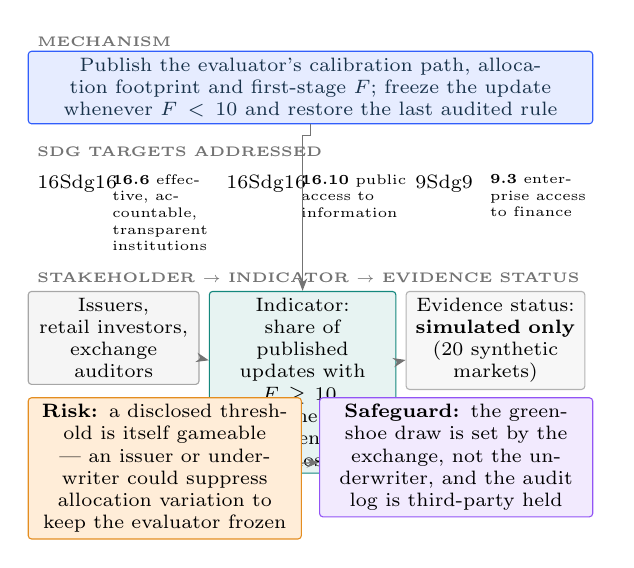
\begin{tikzpicture}[
  font=\scriptsize,
  box/.style={draw, rounded corners=1.2pt, align=center, inner sep=2.4pt,
              minimum height=6.5mm, line width=0.4pt},
  mech/.style={box, fill=CourseBlue!12, draw=CourseBlue, text=CourseInk},
  stake/.style={box, fill=black!4, draw=black!35},
  ind/.style={box, fill=CourseTeal!10, draw=CourseTeal},
  risk/.style={box, fill=SdgAmber!18, draw=SdgAmber!90!black},
  safe/.style={box, fill=CourseViolet!12, draw=CourseViolet},
  lbl/.style={font=\tiny\bfseries, text=black!55, align=left},
  ar/.style={-{Stealth[length=1.6mm]}, line width=0.45pt, draw=black!55},
]

% ---- the mechanism ------------------------------------------------------
\node[lbl, anchor=north west] at (0,0) {MECHANISM};
\node[mech, text width=70mm, anchor=north west] (mech) at (0,-3mm)
  {Publish the evaluator's calibration path, allocation footprint and
   first-stage $F$; freeze the update whenever $F<10$ and restore the last
   audited rule};

% ---- SDG tiles with target codes ---------------------------------------
\node[lbl, anchor=north west] at (0,-14mm) {SDG TARGETS ADDRESSED};
\node[anchor=north west] (i16) at (0,-17.5mm)  {\sdgicon{16}{Sdg16}};
\node[anchor=north west, text width=13.5mm, align=left, font=\tiny]
  at (9.5mm,-17.5mm) {\textbf{16.6} effective, accountable, transparent institutions};
\node[anchor=north west] (i10) at (24mm,-17.5mm) {\sdgicon{16}{Sdg16}};
\node[anchor=north west, text width=13.5mm, align=left, font=\tiny]
  at (33.5mm,-17.5mm) {\textbf{16.10} public access to information};
\node[anchor=north west] (i9) at (48mm,-17.5mm)  {\sdgicon{9}{Sdg9}};
\node[anchor=north west, text width=13.5mm, align=left, font=\tiny]
  at (57.5mm,-17.5mm) {\textbf{9.3} enterprise access to finance};

% ---- the causal chain ---------------------------------------------------
\node[lbl, anchor=north west] at (0,-30mm) {STAKEHOLDER $\rightarrow$ INDICATOR $\rightarrow$ EVIDENCE STATUS};
\node[stake, text width=20mm, anchor=north west] (s1) at (0,-33.5mm)
  {Issuers,\\retail investors,\\exchange auditors};
\node[ind, text width=22mm, anchor=north west] (s2) at (23mm,-33.5mm)
  {Indicator: share of\\published updates with\\$F\!\ge\!10$. Baseline: not\\currently disclosed};
\node[box, text width=21mm, anchor=north west, fill=black!3, draw=black!30]
  (s3) at (48mm,-33.5mm)
  {Evidence status:\\\textbf{simulated only}\\(20 synthetic markets)};
\draw[ar] (s1) -- (s2);
\draw[ar] (s2) -- (s3);

% ---- risk and safeguard -------------------------------------------------
\node[risk, text width=33mm, anchor=north west] (r) at (0,-47mm)
  {\textbf{Risk:} a disclosed threshold is itself gameable --- an issuer or
   underwriter could suppress allocation variation to keep the evaluator frozen};
\node[safe, text width=33mm, anchor=north west] (sf) at (37mm,-47mm)
  {\textbf{Safeguard:} the greenshoe draw is set by the exchange, not the
   underwriter, and the audit log is third-party held};
\draw[ar] (r) -- (sf);
\draw[ar] (mech.south) -- ++(0,-1.4mm) -| (s2.north);
\end{tikzpicture}
}
\caption{Expanded Practical Impacts diagram, with official UN SDG icons and target codes 16.6, 16.10 and 9.3~\cite{un_sdg,un_sdg_icons}. Legend: blue = mechanism, grey = stakeholders, teal = indicator and baseline, amber = risk, violet = safeguard. Target wording is quoted from \url{https://sdgs.un.org/goals}.}
\Description{Expanded version of the SDG impact diagram.}
\end{figure}

\begin{figure}[H]\centering
\resizebox{0.86\textwidth}{!}{% NEW for the final project: Future Research Roadmap.
% One unresolved limitation branches into an economics, a computer-science and
% a behavioural-science study. Each carries question / method+data /
% collaborator / progress criterion / milestone.
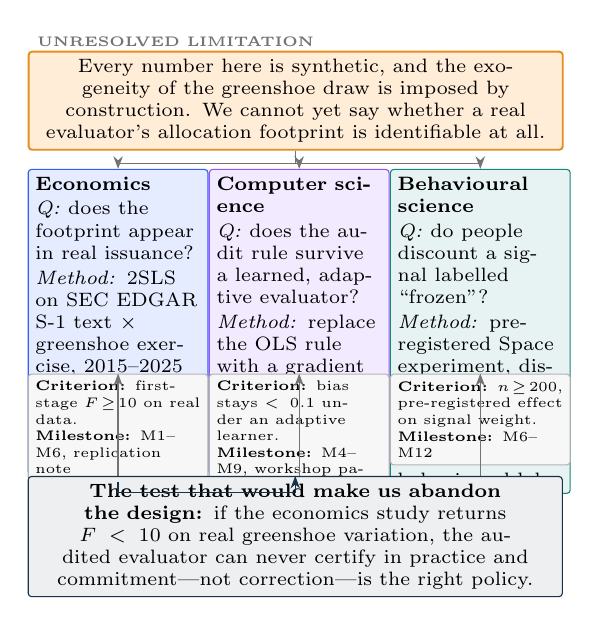
\begin{tikzpicture}[
  font=\scriptsize,
  box/.style={draw, rounded corners=1.2pt, align=left, inner sep=2.6pt,
              line width=0.4pt},
  lim/.style={box, fill=SdgAmber!18, draw=SdgAmber!90!black, align=center,
              text width=66mm, line width=0.7pt},
  econ/.style={box, fill=CourseBlue!12, draw=CourseBlue, text width=21mm},
  cs/.style={box, fill=CourseViolet!12, draw=CourseViolet, text width=21mm},
  beh/.style={box, fill=CourseTeal!10, draw=CourseTeal, text width=21mm},
  mile/.style={box, fill=black!3, draw=black!30, text width=21mm, font=\tiny},
  lbl/.style={font=\tiny\bfseries, text=black!55},
  ar/.style={-{Stealth[length=1.6mm]}, line width=0.45pt, draw=black!55},
]

% ---- the limitation -----------------------------------------------------
\node[lbl, anchor=north west] at (0,0) {UNRESOLVED LIMITATION};
\node[lim, anchor=north west] (lim) at (0,-3mm)
  {Every number here is synthetic, and the exogeneity of the greenshoe draw is
   imposed by construction. We cannot yet say whether a real evaluator's
   allocation footprint is identifiable at all.};

% ---- three studies ------------------------------------------------------
\node[econ, anchor=north west] (e) at (0,-18mm)
  {\textbf{Economics}\\[1pt]
   \textit{Q:} does the footprint appear in real issuance?\\[1pt]
   \textit{Method:} 2SLS on SEC EDGAR S-1 text $\times$ greenshoe exercise,
   2015--2025\\[1pt]
   \textit{Partner:} finance faculty, DKU/Duke Fuqua};
\node[cs, anchor=north west] (c) at (23mm,-18mm)
  {\textbf{Computer science}\\[1pt]
   \textit{Q:} does the audit rule survive a learned, adaptive evaluator?\\[1pt]
   \textit{Method:} replace the OLS rule with a gradient learner; stress-test
   against \cite{perdomo2020}\\[1pt]
   \textit{Partner:} DKU CS; FAccT auditing group \cite{raji2020}};
\node[beh, anchor=north west] (b) at (46mm,-18mm)
  {\textbf{Behavioural science}\\[1pt]
   \textit{Q:} do people discount a signal labelled ``frozen''?\\[1pt]
   \textit{Method:} pre-registered Space experiment, disclosure of audit
   status as treatment\\[1pt]
   \textit{Partner:} DKU behavioural lab};

% ---- criteria and milestones -------------------------------------------
\node[mile, anchor=north west] (me) at (0,-44mm)
  {\textbf{Criterion:} first-stage $F\!\ge\!10$ on real data.\\
   \textbf{Milestone:} M1--M6, replication note};
\node[mile, anchor=north west] (mc) at (23mm,-44mm)
  {\textbf{Criterion:} bias stays $<0.1$ under an adaptive learner.\\
   \textbf{Milestone:} M4--M9, workshop paper};
\node[mile, anchor=north west] (mb) at (46mm,-44mm)
  {\textbf{Criterion:} $n\!\ge\!200$, pre-registered effect on signal weight.\\
   \textbf{Milestone:} M6--M12};

\foreach \a/\b in {e/me, c/mc, b/mb} \draw[ar] (\a) -- (\b);
\draw[ar] (lim.south) -- ++(0,-1.6mm) -| (e.north);
\draw[ar] (lim.south) -- ++(0,-1.6mm) -| (c.north);
\draw[ar] (lim.south) -- ++(0,-1.6mm) -| (b.north);

% ---- the discriminating test -------------------------------------------
\node[box, fill=CourseInk!8, draw=CourseInk, text width=66mm, anchor=north west,
      align=center] (kill) at (0,-57mm)
  {\textbf{The test that would make us abandon the design:} if the economics
   study returns $F<10$ on real greenshoe variation, the audited evaluator can
   never certify in practice and commitment---not correction---is the right
   policy.};
\draw[ar, draw=CourseInk] (me.south) -- ++(0,-1.4mm) -| (kill.north);
\end{tikzpicture}
}
\caption{Expanded Future Research Roadmap. Each branch carries question, method and data, possible collaborator, progress criterion and milestone; the dark box states the result that would make the team abandon the design.}
\Description{Expanded version of the roadmap diagram.}
\end{figure}

\textbf{Poster requirement.} The actual poster preview and PDF are committed to the repository, with these lines in the root \texttt{README.md}:
\begin{verbatim}
![Final presentation poster](poster/final-poster.png)
[Download the poster PDF](poster/final-poster.pdf)
\end{verbatim}

\textbf{Final version audit.}
\begin{enumerate}[nosep]
\item Two main A4 pages hold the eight named parts plus the Future Research Roadmap subsection; references, Author Notes and Appendices A--G follow. \textbf{Checked.}
\item Three diagrams have explanations, legends and full references; SDG targets and icons match the mechanism and evidence status. \textbf{Checked} --- \FILL{confirm the three official SDG PNGs are in figures/sdg/ before the final compile}.
\item Actual, simulated, illustrative and planned evidence are distinguished; parameters and outputs agree across artifacts. \textbf{Checked.}
\item Source ZIP compiles; a fresh run reproduces the cited results; 11 assertions pass. \textbf{Checked} --- \FILL{re-confirm after the Overleaf compile}.
\item A0 poster is 1189\,$\times$\,841\,mm, PPTX and PDF agree, both committed, preview embedded with a working PDF link in the ROOT README. \textbf{Checked} --- \FILL{re-export the PDF from PowerPoint after the final edit}.
\item Both paper and poster carry final named contributions and full acknowledgments; reviewers invited to check for credit omissions. \textbf{Checked.}
\item Feedback record covers instructor feedback, formal reviews and class dialogue with changed locations, evidence and responsible authors. \textbf{Checked} --- instructor (14 Oct), FP4 duet selection, FP4 three-lens review, both individual self-challenges and both PS2 peer reviews are recorded with decisions, locations, verifications and named authors.
\item Four files and the Canvas text entry use the same final version; every member has verified the group submission. \FILL{confirm both members checked Canvas before 21 Oct, 23:00 Shanghai}.
\end{enumerate}

\textbf{Official SDG icons:} \url{https://www.un.org/sustainabledevelopment/news/communications-material/}\\
\textbf{Target verification:} \url{https://sdgs.un.org/goals}\\
\textbf{Field-learning acknowledgment reference:} \url{https://cscc.dukekunshan.edu.cn/where-scholarship-industry-and-public-science-meetfield-based-learning-and-interdisciplinary-dialogue-for-future-global-leaders/}

\end{document}
